%!TEX TS-program = xelatex



\documentclass[a4paper,14pt]{article}


%%% Работа с русским языком
\usepackage[english,russian]{babel}   %% загружает пакет многоязыковой вёрстки
\usepackage{fontspec}      %% подготавливает загрузку шрифтов Open Type, True Type и др.
\defaultfontfeatures{Ligatures={TeX},Renderer=Basic}  %% свойства шрифтов по умолчанию
\setmainfont[Ligatures={TeX,Historic}]{Times New Roman} %% задаёт основной шрифт документа
\setsansfont{Comic Sans MS}                    %% задаёт шрифт без засечек
\setmonofont{Courier New}
\usepackage{indentfirst}
\frenchspacing

\renewcommand{\epsilon}{\ensuremath{\varepsilon}}
\renewcommand{\phi}{\ensuremath{\varphi}}
\renewcommand{\kappa}{\ensuremath{\varkappa}}
\renewcommand{\le}{\ensuremath{\leqslant}}
\renewcommand{\leq}{\ensuremath{\leqslant}}
\renewcommand{\ge}{\ensuremath{\geqslant}}
\renewcommand{\geq}{\ensuremath{\geqslant}}
\renewcommand{\emptyset}{\varnothing}

%%% Дополнительная работа с математикой
\usepackage{amsmath,amsfonts,amssymb,amsthm,mathtools} % AMS
\usepackage{icomma} % "Умная" запятая: $0,2$ --- число, $0, 2$ --- перечисление

%% Номера формул
%\mathtoolsset{showonlyrefs=true} % Показывать номера только у тех формул, на которые есть \eqref{} в тексте.
%\usepackage{leqno} % Нумерация формул слева	

%% Перенос знаков в формулах (по Львовскому)
\newcommand*{\hm}[1]{#1\nobreak\discretionary{}
	{\hbox{$\mathsurround=0pt #1$}}{}}

%%% Работа с картинками
\usepackage{graphicx}  % Для вставки рисунков
\graphicspath{{images/}}  % папки с картинками
\setlength\fboxsep{3pt} % Отступ рамки \fbox{} от рисунка
\setlength\fboxrule{1pt} % Толщина линий рамки \fbox{}
\usepackage{wrapfig} % Обтекание рисунков текстом


%%% Работа с таблицами
\usepackage{array,tabularx,tabulary,booktabs} % Дополнительная работа с таблицами
\usepackage{longtable}  % Длинные таблицы
\usepackage{multirow} % Слияние строк в таблице
\usepackage{float}% http://ctan.org/pkg/float

%%% Программирование
\usepackage{etoolbox} % логические операторы


%%% Страница
\usepackage{extsizes} % Возможность сделать 14-й шрифт
\usepackage{geometry} % Простой способ задавать поля
\geometry{top=20mm}
\geometry{bottom=20mm}
\geometry{left=20mm}
\geometry{right=10mm}
%
%\usepackage{fancyhdr} % Колонтитулы
% 	\pagestyle{fancy}
%\renewcommand{\headrulewidth}{0pt}  % Толщина линейки, отчеркивающей верхний колонтитул
% 	\lfoot{Нижний левый}
% 	\rfoot{Нижний правый}
% 	\rhead{Верхний правый}
% 	\chead{Верхний в центре}
% 	\lhead{Верхний левый}
%	\cfoot{Нижний в центре} % По умолчанию здесь номер страницы

\usepackage{setspace} % Интерлиньяж
\onehalfspacing % Интерлиньяж 1.5
%\doublespacing % Интерлиньяж 2
%\singlespacing % Интерлиньяж 1

\usepackage{lastpage} % Узнать, сколько всего страниц в документе.

\usepackage{soul} % Модификаторы начертания

\usepackage{hyperref}
\usepackage[usenames,dvipsnames,svgnames,table,rgb]{xcolor}
\hypersetup{				% Гиперссылки
	unicode=true,           % русские буквы в раздела PDF
	pdftitle={Заголовок},   % Заголовок
	pdfauthor={Автор},      % Автор
	pdfsubject={Тема},      % Тема
	pdfcreator={Создатель}, % Создатель
	pdfproducer={Производитель}, % Производитель
	pdfkeywords={keyword1} {key2} {key3}, % Ключевые слова
	colorlinks=true,       	% false: ссылки в рамках; true: цветные ссылки
	linkcolor=black,          % внутренние ссылки
	citecolor=black,        % на библиографию
	filecolor=magenta,      % на файлы
	urlcolor=black           % на URL
}
\makeatletter 
\def\@biblabel#1{#1. } 
\makeatother
\usepackage{cite} % Работа с библиографией
%\usepackage[superscript]{cite} % Ссылки в верхних индексах
%\usepackage[nocompress]{cite} % 
\usepackage{csquotes} % Еще инструменты для ссылок

\usepackage{multicol} % Несколько колонок

\usepackage{tikz} % Работа с графикой
\usepackage{pgfplots}
\usepackage{pgfplotstable}

% ГОСТ заголовки
\usepackage[font=small]{caption}
%\captionsetup[table]{justification=centering, labelsep = newline} % Таблицы по правобу краю
%\captionsetup[figure]{justification=centering} % Картинки по центру


\newcommand{\tablecaption}[1]{\addtocounter{table}{1}\small \begin{flushright}\tablename \ \thetable\end{flushright}%	
\begin{center}#1\end{center}}

\newcommand{\imref}[1]{рис.~\ref{#1}}


\usepackage[figure,table,page]{totalcount}
\usepackage{lastpage}
\makeatletter
\long\def\@secondoffour#1#2#3#4{#2}
\def\getlastpage{\ifx\r@LastPage\@undefined 0\else
	\expandafter\@secondoffour\r@LastPage\@empty\@empty\fi}
\makeatother

\usepackage{lipsum}
\usepackage{lastbib}
\begin{document} % конец преамбулы, начало документа
\begin{titlepage}
	\begin{center}
		Правительство Российской Федерации
	\end{center}

	\begin{center}
	Федеральное государственное автономное образовательное учреждение
	Высшего профессионального образования
	
	\end{center}
	
	\begin{center}
		\textbf{Национальный исследовательский университет}
		
		\textbf{«Высшая школа экономики»}
	\end{center}
	%\vspace{1ex}	
	\begin{center}
		МИЭМ
	\end{center}
	\begin{center}
		Департамент электронной инженерии
	\end{center}
	\vspace{1ex}
	\begin{center}
		\textbf{ОТЧЁТ}
		
		По домашней работе
		
		«Проектирование многоразрядного десятичного сумматоракомбинционного типа»
	\end{center}	
	
	\vspace{10ex}
	\begin{flushright}
		\textbf{Студент} группы БИВ-172
		
		Солодянкин Андрей Александрович		
	\end{flushright}
	\vspace{3ex}
	\begin{flushright}
		\textbf{Руководитель} 
		
		Бирюков И.И.

			
	\end{flushright}
	\vfill
	\begin{center}
		Москва \the\year г.
	\end{center}
\end{titlepage}

\section{Исходные данные для проектирования}


\begin{enumerate}
	\item Количество десятичных разрядов: $3$;
	\item Двоично-десятичный код, в котором находятся числа: $2421$;
	\item Система логических элементов: И-НЕ, И;
	\item Критерий оптимальности элементов для проектирования логических схем: минимальное число логических элементов (ЛЭ) в проектируемых схемах;
	\item Тип триггера для проектирования схемы управления синхронный D-треггер;
	\item Временные параметры синхронизирующей серии импульсов логических элементов: 
	время задержки в любом ЛЭ: 1 нс; 
	имульсы синхронизации длительностью 2 нс со скважностью 1. 
\end{enumerate}

\section{Разработка алгоритма выполнения арифметических операций сложения и вычитания многоразрядных чисел в заданом двоично-десятичном коде}

\begin{table}[H]
		\begin{center}

				\caption{\label{tab:alfabet} Двоично-десятичный код 2421 }
	\begin{tabular}{|c|c|}
		\hline
		\multicolumn{1}{|l|}{Цифра} & \multicolumn{1}{l|}{код (2421)} \\ \hline
		0 & 0000 \\ \hline
		1 & 0001 \\ \hline
		2 & 0010 \\ \hline
		3 & 0011 \\ \hline
		4 & 0100 \\ \hline
		5 & 1011 \\ \hline
		6 & 1100 \\ \hline
		7 & 1101 \\ \hline
		8 & 1110 \\ \hline
		9 & 1111 \\ \hline
	\end{tabular}
\end{center}
\end{table}

\subsection{Разработка алгоритма для одноразрядных десятичных чисел, получение величины коррекции и критерии ее ввода}

\begin{table}[H]
		\begin{center}

				\caption{\label{tab:sootv} Таблица соответствия для кода 2421}
	
	\begin{tabular}{|c|c|c|c|c|c|c|c|c|c|c|}
		\hline
		& 0000 & 0001 & 0010 & 0011 & 0100 & 1011 & 1100 & 1101 & 1110 & 1111 \\ \hline
		0000 & \begin{tabular}[c]{@{}c@{}}00000\\ 00000\\ --\end{tabular} & \begin{tabular}[c]{@{}c@{}}0001\\ 0001\\ --\end{tabular} & \begin{tabular}[c]{@{}c@{}}0010\\ 0010\\ --\end{tabular} & \begin{tabular}[c]{@{}c@{}}0011\\ 0011\\ --\end{tabular} & \begin{tabular}[c]{@{}c@{}}0100\\ 0100\\ --\end{tabular} & \begin{tabular}[c]{@{}c@{}}1011\\ 1011\\ --\end{tabular} & \begin{tabular}[c]{@{}c@{}}1100\\ 1100\\ --\end{tabular} & \begin{tabular}[c]{@{}c@{}}1101\\ 1101\\ --\end{tabular} & \begin{tabular}[c]{@{}c@{}}1110\\ 1110\\ --\end{tabular} & \begin{tabular}[c]{@{}c@{}}1111\\ 1111\\ --\end{tabular} \\ \hline
		0001 & \begin{tabular}[c]{@{}c@{}}0001\\ 0001\\ --\end{tabular} & \begin{tabular}[c]{@{}c@{}}0010\\ 0010\\ --\end{tabular} & \begin{tabular}[c]{@{}c@{}}0011\\ 0011\\ --\end{tabular} & \begin{tabular}[c]{@{}c@{}}0100\\ 0100\\ --\end{tabular} & \begin{tabular}[c]{@{}c@{}}0101\\ 1011\\ 0110\end{tabular} & \begin{tabular}[c]{@{}c@{}}1100\\ 1100\\ --\end{tabular} & \begin{tabular}[c]{@{}c@{}}1101\\ 1101\\ --\end{tabular} & \begin{tabular}[c]{@{}c@{}}1110\\ 1110\\ --\end{tabular} & \begin{tabular}[c]{@{}c@{}}1111\\ 1111\\ --\end{tabular} & \begin{tabular}[c]{@{}c@{}}0000\\ 0000\\ --\end{tabular} \\ \hline
		0010 & \begin{tabular}[c]{@{}c@{}}0010\\ 0010\\ --\end{tabular} & \begin{tabular}[c]{@{}c@{}}0011\\ 0011\\ --\end{tabular} & \begin{tabular}[c]{@{}c@{}}0100\\ 0100\\ --\end{tabular} & \begin{tabular}[c]{@{}c@{}}0101\\ 1011\\ 0110\end{tabular} & \begin{tabular}[c]{@{}c@{}}0110\\ 1100\\ 0110\end{tabular} & \begin{tabular}[c]{@{}c@{}}1101\\ 1101\\ --\end{tabular} & \begin{tabular}[c]{@{}c@{}}1110\\ 1110\\ --\end{tabular} & \begin{tabular}[c]{@{}c@{}}1111\\ 1111\\ --\end{tabular} & \begin{tabular}[c]{@{}c@{}}0000\\ 0000\\ --\end{tabular} & \begin{tabular}[c]{@{}c@{}}0001\\ 0001\\ --\end{tabular} \\ \hline
		0011 & \begin{tabular}[c]{@{}c@{}}0011\\ 0011\\ --\end{tabular} & \begin{tabular}[c]{@{}c@{}}0100\\ 0100\\ --\end{tabular} & \begin{tabular}[c]{@{}c@{}}0101\\ 1011\\ 0110\end{tabular} & \begin{tabular}[c]{@{}c@{}}0110\\ 1100\\ 0110\end{tabular} & \begin{tabular}[c]{@{}c@{}}0111\\ 1101\\ 0110\end{tabular} & \begin{tabular}[c]{@{}c@{}}1110\\ 1110\\ --\end{tabular} & \begin{tabular}[c]{@{}c@{}}1111\\ 1111\\ --\end{tabular} & \begin{tabular}[c]{@{}c@{}}0000\\ 0000\\ --\end{tabular} & \begin{tabular}[c]{@{}c@{}}0001\\ 0001\\ --\end{tabular} & \begin{tabular}[c]{@{}c@{}}0010\\ 0010\\ --\end{tabular} \\ \hline
		0100 & \begin{tabular}[c]{@{}c@{}}0100\\ 0100\\ --\end{tabular} & \begin{tabular}[c]{@{}c@{}}0101\\ 1011\\ 0110\end{tabular} & \begin{tabular}[c]{@{}c@{}}0110\\ 1100\\ 0110\end{tabular} & \begin{tabular}[c]{@{}c@{}}0111\\ 1101\\ 0110\end{tabular} & \begin{tabular}[c]{@{}c@{}}1000\\ 1110\\ 0110\end{tabular} & \begin{tabular}[c]{@{}c@{}}1111\\ 1111\\ --\end{tabular} & \begin{tabular}[c]{@{}c@{}}0000\\ 0000\\ --\end{tabular} & \begin{tabular}[c]{@{}c@{}}0001\\ 0001\\ --\end{tabular} & \begin{tabular}[c]{@{}c@{}}0010\\ 0010\\ --\end{tabular} & \begin{tabular}[c]{@{}c@{}}0011\\ 0011\\ --\end{tabular} \\ \hline
		1011 & \begin{tabular}[c]{@{}c@{}}1011\\ 1011\\ --\end{tabular} & \begin{tabular}[c]{@{}c@{}}1100\\ 1100\\ --\end{tabular} & \begin{tabular}[c]{@{}c@{}}1101\\ 1101\\ --\end{tabular} & \begin{tabular}[c]{@{}c@{}}1110\\ 1110\\ --\end{tabular} & \begin{tabular}[c]{@{}c@{}}1111\\ 1111\\ --\end{tabular} & \begin{tabular}[c]{@{}c@{}}0110\\ 0000\\ 1010\end{tabular} & \begin{tabular}[c]{@{}c@{}}0111\\ 0001\\ 1010\end{tabular} & \begin{tabular}[c]{@{}c@{}}1000\\ 0010\\ 1010\end{tabular} & \begin{tabular}[c]{@{}c@{}}1001\\ 0011\\ 1010\end{tabular} & \begin{tabular}[c]{@{}c@{}}1010\\ 0100\\ 1010\end{tabular} \\ \hline
		1100 & \begin{tabular}[c]{@{}c@{}}1100\\ 1100\\ --\end{tabular} & \begin{tabular}[c]{@{}c@{}}1101\\ 1101\\ --\end{tabular} & \begin{tabular}[c]{@{}c@{}}1110\\ 1110\\ --\end{tabular} & \begin{tabular}[c]{@{}c@{}}1111\\ 1111\\ --\end{tabular} & \begin{tabular}[c]{@{}c@{}}0000\\ 0000\\ --\end{tabular} & \begin{tabular}[c]{@{}c@{}}0111\\ 0001\\ 1010\end{tabular} & \begin{tabular}[c]{@{}c@{}}1000\\ 0010\\ 1010\end{tabular} & \begin{tabular}[c]{@{}c@{}}1001\\ 0011\\ 1010\end{tabular} & \begin{tabular}[c]{@{}c@{}}1010\\ 0100\\ 1010\end{tabular} & \begin{tabular}[c]{@{}c@{}}1011\\ 1011\\ --\end{tabular} \\ \hline
		1101 & \begin{tabular}[c]{@{}c@{}}1101\\ 1101\\ --\end{tabular} & \begin{tabular}[c]{@{}c@{}}1110\\ 1110\\ --\end{tabular} & \begin{tabular}[c]{@{}c@{}}1111\\ 1111\\ --\end{tabular} & \begin{tabular}[c]{@{}c@{}}0000\\ 0000\\ --\end{tabular} & \begin{tabular}[c]{@{}c@{}}0001\\ 0001\\ --\end{tabular} & \begin{tabular}[c]{@{}c@{}}1000\\ 0010\\ 1010\end{tabular} & \begin{tabular}[c]{@{}c@{}}1001\\ 0011\\ 1010\end{tabular} & \begin{tabular}[c]{@{}c@{}}1010\\ 0100\\ 1010\end{tabular} & \begin{tabular}[c]{@{}c@{}}1011\\ 1011\\ --\end{tabular} & \begin{tabular}[c]{@{}c@{}}1100\\ 1100\\ --\end{tabular} \\ \hline
		1110 & \begin{tabular}[c]{@{}c@{}}1110\\ 1110\\ --\end{tabular} & \begin{tabular}[c]{@{}c@{}}1111\\ 1111\\ --\end{tabular} & \begin{tabular}[c]{@{}c@{}}0000\\ 0000\\ --\end{tabular} & \begin{tabular}[c]{@{}c@{}}0001\\ 0001\\ --\end{tabular} & \begin{tabular}[c]{@{}c@{}}0010\\ 0010\\ --\end{tabular} & \begin{tabular}[c]{@{}c@{}}1001\\ 0011\\ 1010\end{tabular} & \begin{tabular}[c]{@{}c@{}}1010\\ 0100\\ 1010\end{tabular} & \begin{tabular}[c]{@{}c@{}}1011\\ 1011\\ --\end{tabular} & \begin{tabular}[c]{@{}c@{}}1100\\ 1100\\ --\end{tabular} & \begin{tabular}[c]{@{}c@{}}1101\\ 1101\\ --\end{tabular} \\ \hline
		1111 & \begin{tabular}[c]{@{}c@{}}1111\\ 1111\\ --\end{tabular} & \begin{tabular}[c]{@{}c@{}}0000\\ 0000\\ --\end{tabular} & \begin{tabular}[c]{@{}c@{}}0001\\ 0001\\ --\end{tabular} & \begin{tabular}[c]{@{}c@{}}0010\\ 0010\\ --\end{tabular} & \begin{tabular}[c]{@{}c@{}}0011\\ 0011\\ --\end{tabular} & \begin{tabular}[c]{@{}c@{}}1010\\ 0100\\ 1010\end{tabular} & \begin{tabular}[c]{@{}c@{}}1011\\ 1011\\ --\end{tabular} & \begin{tabular}[c]{@{}c@{}}1100\\ 1100\\ --\end{tabular} & \begin{tabular}[c]{@{}c@{}}1101\\ 1101\\ --\end{tabular} & \begin{tabular}[c]{@{}c@{}}1110\\ 1110\\ --\end{tabular} \\ \hline
	\end{tabular}
\end{center}
\end{table}

Критерии ввода корректировки:

\begin{itemize}
	\item Если получена разрешенная комбинация и вне зависимости от наличия единицы переноса, корректировка не вводится, при этом единица переноса сохраняется;
	\item Если получена запрещенная комбинация и нет единицы переноса, то вводится корректировка $0110$;
	\item Если получена запрещенная комбинация и есть единица переноса, то вводится корректировка $1010$, при этом единица переноса сохраняется;
\end{itemize}

\subsection{Обобщение полученного алгоритма на многоразрядные числа при выполнении операции сложения и вычитания}

\subsection{Приведение шести примеров на следующие случаи сложения}

%Положительная величина (+A) складывается с другой положительной величиной (+B) с получением положительного результата (+C) без переполнения 
\subsubsection{(+A)+(+B)=(+C)}

%\begin{figure}[H]
%	\centering
%	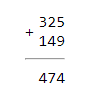
\includegraphics[width=0.2\linewidth]{images/2_3_1_01}
%	\caption{}
%	\label{fig:23101}
%\end{figure}

\begin{figure}[H]
	\centering
	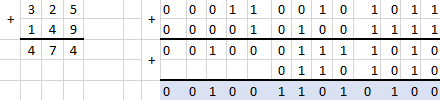
\includegraphics[width=0.7\linewidth]{primeri/screenshot001}
	\caption{}
	\label{fig:screenshot001}
\end{figure}



\subsubsection{(+A)+(-B)=(+C)}

%\begin{figure}[H]
%	\centering
%	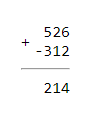
\includegraphics[width=0.4\linewidth]{images/2_3_2_01}
%	\caption{}
%	\label{fig:23201}
%\end{figure}

\begin{figure}[H]
	\centering
	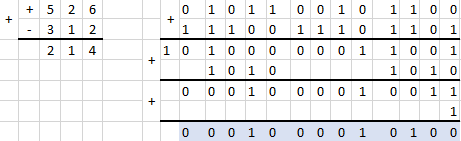
\includegraphics[width=0.7\linewidth]{primeri/screenshot002}
	\caption{}
	\label{fig:screenshot002}
\end{figure}


\subsubsection{(+A)+(-B)=(-C)}

%\begin{figure}[H]
%	\centering
%	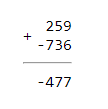
\includegraphics[width=0.4\linewidth]{images/2_3_3_01}
%	\caption{}
%	\label{fig:23301}
%\end{figure}

\begin{figure}[H]
	\centering
	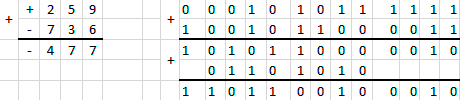
\includegraphics[width=0.7\linewidth]{primeri/pr_3_2}
	\caption{}
	\label{fig:screenshot003}
\end{figure}

\subsubsection{(-A)+(-B)=(-C)}

%\begin{figure}[H]
%	\centering
%	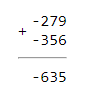
\includegraphics[width=0.4\linewidth]{images/2_3_4_01}
%	\caption{}
%	\label{fig:23401}
%\end{figure}

\begin{figure}[H]
	\centering
	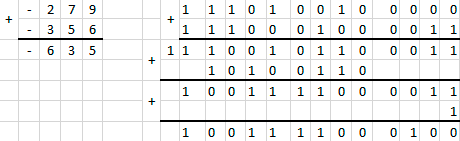
\includegraphics[width=0.7\linewidth]{primeri/pr_4_2}
	\caption{}
	\label{fig:screenshot004}
\end{figure}

\subsubsection{(+A)+(+B)=(-C) — Переполнение разрядной сетки}

%\begin{figure}[H]
%	\centering
%	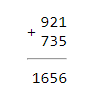
\includegraphics[width=0.4\linewidth]{images/2_3_5_01}
%	\caption{}
%	\label{fig:23501}
%\end{figure}

\begin{figure}[H]
	\centering
	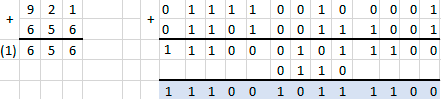
\includegraphics[width=0.7\linewidth]{primeri/screenshot005}
	\caption{}
	\label{fig:screenshot005}
\end{figure}


\subsubsection{(-A)+(-B)=(+C) — Переполнение разрядной сетки}

%\begin{figure}[H]
%	\centering
%	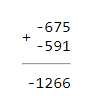
\includegraphics[width=0.4\linewidth]{images/2_3_6_01}
%	\caption{}
%	\label{fig:23601}
%\end{figure}

\begin{figure}[H]
	\centering
	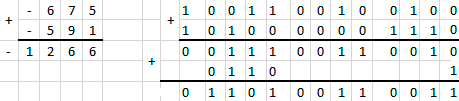
\includegraphics[width=0.7\linewidth]{primeri/pr_6_2}
	\caption{}
	\label{fig:screenshot006}
\end{figure}

\section{Разработки функциональной схемы одноразрядного десятичного сумматора комбинационного типа}

\subsection{Разработка оптимальной схемы (с точки зрения критерия оптимальности) одноразрядного двоичного сумматора с учетом заданного базиса логических элементов}

Разработаем схему одноразрядного двоичного сумматора в базисе И, И-НЕ.

\begin{figure}[H]
	\centering
	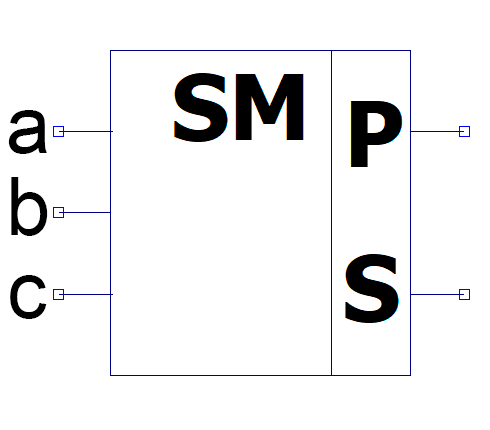
\includegraphics[width=0.3\linewidth]{images/dvSum_el}
	\caption{одноразрядный двоичный сумматор}
	\label{fig:dvSum_el}
\end{figure}

$a$ -- перовое слагаемое;

$b$ -- второе слагаемое;

$c$ -- перенос из соседнего младшего разряда;

$S$ -- сумма в данном разряде;

$P$ -- перенос в соседний старший разряд.

В дальнейшем одноразрядный двоичный сумматор будет обозначаться как на рисунке \ref{fig:dvSum_el}.

\begin{table}[H]
\begin{center}
	\caption{\label{tab:dvSum} Таблица истинности для функций $S$ и $P$ суммы и перенса в однороразрядном двоичном сумматоре}
	\begin{tabular}{|l|l|l|l|l|}
		\hline
		$a$ & $b$ & $c$ & $S$ & $P$ \\ \hline
		0 & 0 & 0 & 0 & 0 \\ \hline
		0 & 0 & 1 & 1 & 0 \\ \hline
		0 & 1 & 0 & 1 & 0 \\ \hline
		0 & 1 & 1 & 0 & 1 \\ \hline
		1 & 0 & 0 & 1 & 0 \\ \hline
		1 & 0 & 1 & 0 & 1 \\ \hline
		1 & 1 & 0 & 0 & 1 \\ \hline
		1 & 1 & 1 & 1 & 1 \\ \hline
	\end{tabular}
\end{center}
\end{table}

\begin{table}[H]
	\begin{center}
		\caption{\label{tab:SDvSum} Диаграмма Вейча для функции $S$}
	\begin{tabular}{ccccc}
		& \multicolumn{2}{c}{$a$}                           & \multicolumn{2}{c}{$\overline{a}$}                          \\ \cline{2-5} 
		\multicolumn{1}{c|}{$b$}  & \multicolumn{1}{c|}{}  & \multicolumn{1}{c|}{1} & \multicolumn{1}{c|}{}  & \multicolumn{1}{c|}{1} \\ \cline{2-5} 
		\multicolumn{1}{c|}{$\overline{b}$} & \multicolumn{1}{c|}{1} & \multicolumn{1}{c|}{}  & \multicolumn{1}{c|}{1} & \multicolumn{1}{c|}{}  \\ \cline{2-5} 
		&$\overline{c}$                   & \multicolumn{2}{c}{$c$}                          & $\overline{c}$                    
	\end{tabular}
\end{center}
\end{table}

Для создания логической схемы в базисе И, И-НЕ необходима диаграмма Вейча для функции $\overline{S}$.

\begin{table}[H]
	\begin{center}
		\caption{\label{tab:NSDvSum} Диаграмма Вейча для функции $\overline{S}$}
		\begin{tabular}{ccccc}
			& \multicolumn{2}{c}{$a$}                           & \multicolumn{2}{c}{$\overline{a}$}                          \\ \cline{2-5} 
			\multicolumn{1}{c|}{$b$}  & \multicolumn{1}{c|}{1}  & \multicolumn{1}{c|}{} & \multicolumn{1}{c|}{1}  & \multicolumn{1}{c|}{} \\ \cline{2-5} 
			\multicolumn{1}{c|}{$\overline{b}$} & \multicolumn{1}{c|}{} & \multicolumn{1}{c|}{1}  & \multicolumn{1}{c|}{} & \multicolumn{1}{c|}{1}  \\ \cline{2-5} 
			& $\overline{c}$      & \multicolumn{2}{c}{$c$}                          &$\overline{c}$                   
		\end{tabular}
	\end{center}
\end{table}

$$\overline{S} = ab\bar{c} + a\bar{b}c + \bar{a}bc + \bar{a}\bar{b}\bar{c}$$

$$S = \overline{ab\bar{c} + a\bar{b}c + \bar{a}bc + \bar{a}\bar{b}\bar{c}}$$

$$S = \overline{ab\bar{c}} * \overline{a\bar{b}c} * \overline{\bar{a}bc} * \overline{\bar{a}\bar{b}\bar{c}}$$

 В дальнейшем будем сразу строить диаграммы Вйеча для обратных функций.
 
 \begin{table}[H]
 	\begin{center}
 		\caption{\label{tab:NPDvSum} Диаграмма Вейча для функции $\overline{P}$}
 		\begin{tabular}{ccccc}
 			& \multicolumn{2}{c}{$a$}                           & \multicolumn{2}{c}{$\overline{a}$}                          \\ \cline{2-5} 
 			\multicolumn{1}{c|}{$b$}  & \multicolumn{1}{c|}{}  & \multicolumn{1}{c|}{} & \multicolumn{1}{c|}{}  & \multicolumn{1}{c|}{1} \\ \cline{2-5} 
 			\multicolumn{1}{c|}{$\overline{b}$} & \multicolumn{1}{c|}{1} & \multicolumn{1}{c|}{}  & \multicolumn{1}{c|}{1} & \multicolumn{1}{c|}{1}  \\ \cline{2-5} 
 			& $\overline{c}$                   & \multicolumn{2}{c}{$c$}                          & $\overline{c}$               
 		\end{tabular}
 	\end{center}
 \end{table}

$$\overline{P} = \bar{b}\bar{c} + \bar{a}\bar{b} + \bar{a}\bar{c}$$

$$P = \overline{ \bar{b}\bar{c} + \bar{a}\bar{b} + \bar{a}\bar{c}}$$

$$ P = \overline{ \bar{b}\bar{c}} *  \overline{ \bar{a}\bar{b}} * \overline{ \bar{a}\bar{c}}$$

\begin{figure}[H]
	\centering
	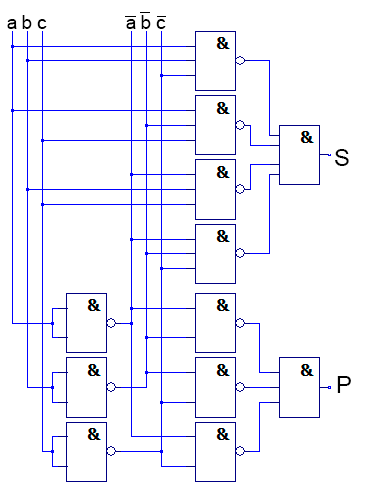
\includegraphics[width=0.5\linewidth]{images/dvSum_sh}
	\caption{Логическая схема одноразрядного двоичного сумматора}
	\label{fig:dvSum_sh}
\end{figure}

\subsection{Разработка схемы коррекции}

Разработаем корректор.

\begin{figure}[H]
	\centering
	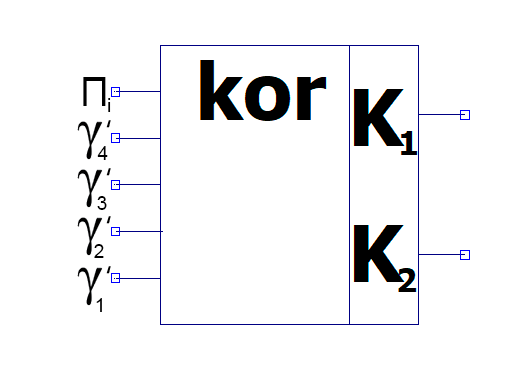
\includegraphics[width=0.3\linewidth]{images/korr_el}
	\caption{корректор}
	\label{fig:korr_el}
\end{figure}

$\gamma_4, \gamma_3, \gamma_2, \gamma_1$ -- тетрада до корекции;

$\Pi_i$ -- перенос в следующую тетраду.

\begin{table}[H]
	\begin{center}
		\caption{\label{tab:dvKorr} Таблица истинности для функций $K_1$ и $K_2$ в корректоре}
	\begin{tabular}{|l|l|l|l|l|l|l|}
		\hline
		$\gamma_4$ & $\gamma_3$ & $\gamma_2$ & $\gamma_1$ & П & K1 & K2 \\ \hline
		0  & 0  & 0  & 0  & 0 & 0  & 0  \\ \hline
		0  & 0  & 0  & 0  & 1 & 0  & 0  \\ \hline
		0  & 0  & 0  & 1  & 0 & 0  & 0  \\ \hline
		0  & 0  & 0  & 1  & 1 & 0  & 0  \\ \hline
		0  & 0  & 1  & 0  & 0 & 0  & 0  \\ \hline
		0  & 0  & 1  & 0  & 1 & 0  & 0  \\ \hline
		0  & 0  & 1  & 1  & 0 & 0  & 0  \\ \hline
		0  & 0  & 1  & 1  & 1 & 0  & 0  \\ \hline
		0  & 1  & 0  & 0  & 0 & 0  & 0  \\ \hline
		0  & 1  & 0  & 0  & 1 & 0  & 0  \\ \hline
		0  & 1  & 0  & 1  & 0 & 1  & 0  \\ \hline
		0  & 1  & 0  & 1  & 1 & x  & x  \\ \hline
		0  & 1  & 1  & 0  & 0 & 1  & 0  \\ \hline
		0  & 1  & 1  & 0  & 1 & 0  & 1  \\ \hline
		0  & 1  & 1  & 1  & 0 & 1  & 0  \\ \hline
		0  & 1  & 1  & 1  & 1 & 0  & 1  \\ \hline
		1  & 0  & 0  & 0  & 0 & 1  & 0  \\ \hline
		1  & 0  & 0  & 0  & 1 & 0  & 1  \\ \hline
		1  & 0  & 0  & 1  & 0 & x  & x  \\ \hline
		1  & 0  & 0  & 1  & 1 & 0  & 1  \\ \hline
		1  & 0  & 1  & 0  & 0 & x  & x  \\ \hline
		1  & 0  & 1  & 0  & 1 & 0  & 1  \\ \hline
		1  & 0  & 1  & 1  & 0 & 0  & 0  \\ \hline
		1  & 0  & 1  & 1  & 1 & 0  & 0  \\ \hline
		1  & 1  & 0  & 0  & 0 & 0  & 0  \\ \hline
		1  & 1  & 0  & 0  & 1 & 0  & 0  \\ \hline
		1  & 1  & 0  & 1  & 0 & 0  & 0  \\ \hline
		1  & 1  & 0  & 1  & 1 & 0  & 0  \\ \hline
		1  & 1  & 1  & 0  & 0 & 0  & 0  \\ \hline
		1  & 1  & 1  & 0  & 1 & 0  & 0  \\ \hline
		1  & 1  & 1  & 1  & 0 & 0  & 0  \\ \hline
		1  & 1  & 1  & 1  & 1 & 0  & 0  \\ \hline
	\end{tabular}
\end{center}
\end{table}

\begin{table}[H]
	\begin{center}
		\caption{\label{tab:dvKorrK1} Диаграмма Вейча для функции $K_1$}
	\begin{tabular}{cccccccccc}
		& \multicolumn{4}{c}{$\Pi$}                                                                          & \multicolumn{4}{c}{$\overline{\Pi}$}                                                                            &                     \\
		& \multicolumn{2}{c}{$\gamma_4$}                        & \multicolumn{2}{c}{$\overline{\gamma_4}$}                        & \multicolumn{2}{c}{$\gamma_4$}                          & \multicolumn{2}{c}{$\overline{\gamma_4}$}                         &                     \\ \cline{2-9}
		\multicolumn{1}{c|}{\multirow{2}{*}{$\gamma_3$}}  & \multicolumn{1}{c|}{} & \multicolumn{1}{c|}{} & \multicolumn{1}{c|}{} & \multicolumn{1}{c|}{}  & \multicolumn{1}{c|}{}  & \multicolumn{1}{c|}{}  & \multicolumn{1}{c|}{1} & \multicolumn{1}{c|}{}  & $\overline{\gamma_1}$                 \\ \cline{2-9}
		\multicolumn{1}{c|}{}                     & \multicolumn{1}{c|}{} & \multicolumn{1}{c|}{} & \multicolumn{1}{c|}{} & \multicolumn{1}{c|}{x} & \multicolumn{1}{c|}{}  & \multicolumn{1}{c|}{}  & \multicolumn{1}{c|}{1} & \multicolumn{1}{c|}{1} & \multirow{2}{*}{$\gamma_1$} \\ \cline{2-9}
		\multicolumn{1}{c|}{\multirow{2}{*}{$\overline{\gamma_3}$}} & \multicolumn{1}{c|}{} & \multicolumn{1}{c|}{} & \multicolumn{1}{c|}{} & \multicolumn{1}{c|}{}  & \multicolumn{1}{c|}{x} & \multicolumn{1}{c|}{}  & \multicolumn{1}{c|}{}  & \multicolumn{1}{c|}{}  &                     \\ \cline{2-9}
		\multicolumn{1}{c|}{}                     & \multicolumn{1}{c|}{} & \multicolumn{1}{c|}{} & \multicolumn{1}{c|}{} & \multicolumn{1}{c|}{}  & \multicolumn{1}{c|}{1} & \multicolumn{1}{c|}{x} & \multicolumn{1}{c|}{}  & \multicolumn{1}{c|}{}  & $\overline{\gamma_1}$                 \\ \cline{2-9}
		& $\overline{\gamma_2}$                   & \multicolumn{2}{c}{$\gamma_2$}                        & \multicolumn{2}{c}{$\overline{\gamma_2}$}                         & \multicolumn{2}{c}{$\gamma_2$}                          & $\overline{\gamma_2}$                    &                    
	\end{tabular}
\end{center}
\end{table}

\begin{table}[H]
	\begin{center}
		\caption{\label{tab:dvKorrNK1} Диаграмма Вейча для функции $\overline{K_1}$}
	\begin{tabular}{cccccccccc}
		& \multicolumn{4}{c}{$\Pi$}                                                                             & \multicolumn{4}{c}{$\overline{\Pi}$}                                                                            &                     \\
		& \multicolumn{2}{c}{$\gamma_4$}                          & \multicolumn{2}{c}{$\overline{\gamma_4}$}                         & \multicolumn{2}{c}{$\gamma_4$}                          & \multicolumn{2}{c}{$\overline{\gamma_4}$}                         &                     \\ \cline{2-9}
		\multicolumn{1}{c|}{\multirow{2}{*}{$\gamma_3$}}  & \multicolumn{1}{c|}{1} & \multicolumn{1}{c|}{1} & \multicolumn{1}{c|}{1} & \multicolumn{1}{c|}{1} & \multicolumn{1}{c|}{1} & \multicolumn{1}{c|}{1} & \multicolumn{1}{c|}{}  & \multicolumn{1}{c|}{1} &       $\overline{\gamma_1}$           \\ \cline{2-9}
		\multicolumn{1}{c|}{}                     & \multicolumn{1}{c|}{1} & \multicolumn{1}{c|}{1} & \multicolumn{1}{c|}{1} & \multicolumn{1}{c|}{x} & \multicolumn{1}{c|}{1} & \multicolumn{1}{c|}{1} & \multicolumn{1}{c|}{}  & \multicolumn{1}{c|}{}  & \multirow{2}{*}{$\gamma_1$} \\ \cline{2-9}
		\multicolumn{1}{c|}{\multirow{2}{*}{$\overline{\gamma_3}$}} & \multicolumn{1}{c|}{1} & \multicolumn{1}{c|}{1} & \multicolumn{1}{c|}{1} & \multicolumn{1}{c|}{1} & \multicolumn{1}{c|}{x} & \multicolumn{1}{c|}{1} & \multicolumn{1}{c|}{1} & \multicolumn{1}{c|}{1} &                     \\ \cline{2-9}
		\multicolumn{1}{c|}{}                     & \multicolumn{1}{c|}{1} & \multicolumn{1}{c|}{1} & \multicolumn{1}{c|}{1} & \multicolumn{1}{c|}{1} & \multicolumn{1}{c|}{}  & \multicolumn{1}{c|}{x} & \multicolumn{1}{c|}{1} & \multicolumn{1}{c|}{1} & $\overline{\gamma_1}$                 \\ \cline{2-9}
		& $\overline{\gamma_2}$                    & \multicolumn{2}{c}{$\gamma_2$}                          & \multicolumn{2}{c}{$\overline{\gamma_2}$}                         & \multicolumn{2}{c}{$\gamma_2$}                          & $\overline{\gamma_2}$                    &                    
	\end{tabular}
\end{center}
\end{table}

$$\overline{K_1} = \Pi + \gamma_3 \gamma_4 + \bar{\gamma_3} \bar{\gamma_4} + \gamma_1 \gamma_2 \bar{\gamma_3} + \bar{\gamma_1} \bar{\gamma_2} \gamma_3$$

$$K_1 = \overline{\Pi} * \overline{\gamma_3 \gamma_4} * \overline{\bar{\gamma_3} \bar{\gamma_4}} * \overline{\gamma_1 \gamma_2 \bar{\gamma_3}} * \overline{\bar{\gamma_1} \bar{\gamma_2} \gamma_3}$$





\begin{table}[H]	
	\begin{center}
		\caption{\label{tab:dvKorrK2} Диаграмма Вейча для функции $K_2$}
	\begin{tabular}{cccccccccc}
		& \multicolumn{4}{c}{$\Pi$}                                                                             & \multicolumn{4}{c}{$\overline{\Pi}$}                                                                          &                     \\
		& \multicolumn{2}{c}{$\gamma_4$}                          & \multicolumn{2}{c}{$\overline{\gamma_4}$}                         & \multicolumn{2}{c}{$\gamma_4$}                          & \multicolumn{2}{c}{$\overline{\gamma_4}$}                       &                     \\ \cline{2-9}
		\multicolumn{1}{c|}{\multirow{2}{*}{$\gamma_4$}}  & \multicolumn{1}{c|}{}  & \multicolumn{1}{c|}{}  & \multicolumn{1}{c|}{1} & \multicolumn{1}{c|}{}  & \multicolumn{1}{c|}{}  & \multicolumn{1}{c|}{}  & \multicolumn{1}{c|}{} & \multicolumn{1}{c|}{} & $\overline{\gamma_1}$                 \\ \cline{2-9}
		\multicolumn{1}{c|}{}                     & \multicolumn{1}{c|}{}  & \multicolumn{1}{c|}{}  & \multicolumn{1}{c|}{1} & \multicolumn{1}{c|}{x} & \multicolumn{1}{c|}{}  & \multicolumn{1}{c|}{}  & \multicolumn{1}{c|}{} & \multicolumn{1}{c|}{} & \multirow{2}{*}{$\gamma_1$} \\ \cline{2-9}
		\multicolumn{1}{c|}{\multirow{2}{*}{$\overline{\gamma_3}$}} & \multicolumn{1}{c|}{1} & \multicolumn{1}{c|}{}  & \multicolumn{1}{c|}{}  & \multicolumn{1}{c|}{}  & \multicolumn{1}{c|}{x} & \multicolumn{1}{c|}{}  & \multicolumn{1}{c|}{} & \multicolumn{1}{c|}{} &                     \\ \cline{2-9}
		\multicolumn{1}{c|}{}                     & \multicolumn{1}{c|}{1} & \multicolumn{1}{c|}{1} & \multicolumn{1}{c|}{}  & \multicolumn{1}{c|}{}  & \multicolumn{1}{c|}{}  & \multicolumn{1}{c|}{x} & \multicolumn{1}{c|}{} & \multicolumn{1}{c|}{} & $\overline{\gamma_1}$                \\ \cline{2-9}
		& $\overline{\gamma_2}$                    & \multicolumn{2}{c}{$\gamma_2$}                          & \multicolumn{2}{c}{$\overline{\gamma_2}$}                         & \multicolumn{2}{c}{$\gamma_2$}                         & $\overline{\gamma_2}$                   &                    
	\end{tabular}
\end{center}
\end{table}

\begin{table}[H]
		\begin{center}
		\caption{\label{tab:dvKorrNK2} Диаграмма Вейча для функции $\overline{K_2}$}
	\begin{tabular}{cccccccccc}
		& \multicolumn{4}{c}{$\Pi$}                                                                             & \multicolumn{4}{c}{$\overline{\Pi}$}                                                                            &                     \\
		& \multicolumn{2}{c}{$\gamma_4$}                          & \multicolumn{2}{c}{$\overline{\gamma_4}$}                         & \multicolumn{2}{c}{$\gamma_4$}                          & \multicolumn{2}{c}{$\overline{\gamma_4}$}                         &                     \\ \cline{2-9}
		\multicolumn{1}{c|}{\multirow{2}{*}{$\gamma_4$}}  & \multicolumn{1}{c|}{1} & \multicolumn{1}{c|}{1} & \multicolumn{1}{c|}{}  & \multicolumn{1}{c|}{1} & \multicolumn{1}{c|}{1} & \multicolumn{1}{c|}{1} & \multicolumn{1}{c|}{1} & \multicolumn{1}{c|}{1} & $\overline{\gamma_1}$                 \\ \cline{2-9}
		\multicolumn{1}{c|}{}                     & \multicolumn{1}{c|}{1} & \multicolumn{1}{c|}{1} & \multicolumn{1}{c|}{}  & \multicolumn{1}{c|}{x} & \multicolumn{1}{c|}{1} & \multicolumn{1}{c|}{1} & \multicolumn{1}{c|}{1} & \multicolumn{1}{c|}{1} & \multirow{2}{*}{$\gamma_1$} \\ \cline{2-9}
		\multicolumn{1}{c|}{\multirow{2}{*}{$\overline{\gamma_3}$}} & \multicolumn{1}{c|}{}  & \multicolumn{1}{c|}{1} & \multicolumn{1}{c|}{1} & \multicolumn{1}{c|}{1} & \multicolumn{1}{c|}{x} & \multicolumn{1}{c|}{1} & \multicolumn{1}{c|}{1} & \multicolumn{1}{c|}{1} &                     \\ \cline{2-9}
		\multicolumn{1}{c|}{}                     & \multicolumn{1}{c|}{}  & \multicolumn{1}{c|}{}  & \multicolumn{1}{c|}{1} & \multicolumn{1}{c|}{1} & \multicolumn{1}{c|}{1} & \multicolumn{1}{c|}{x} & \multicolumn{1}{c|}{1} & \multicolumn{1}{c|}{1} & $\overline{\gamma_1}$                \\ \cline{2-9}
		&$\overline{\gamma_2}$               & \multicolumn{2}{c}{$\gamma_2$}                          & \multicolumn{2}{c}{$\overline{\gamma_2}$}                         & \multicolumn{2}{c}{$\gamma_2$}                          & $\overline{\gamma_2}$                   &                    
	\end{tabular}
\end{center}
\end{table}

$$\overline{K_2} = \overline{\Pi} + \gamma_3 \gamma_4 + \bar{\gamma_3} \bar{\gamma_4} + \gamma_1 \gamma_2 \bar{\gamma_3} + \bar{\gamma_1} \bar{\gamma_2} \gamma_3$$

$$K_2 = \Pi * \overline{\gamma_3 \gamma_4} * \overline{\bar{\gamma_3} \bar{\gamma_4}} * \overline{\gamma_1 \gamma_2 \bar{\gamma_3}} * \overline{\bar{\gamma_1} \bar{\gamma_2} \gamma_3}$$

Можно заменить, что для функций $K1$ и $K2$ есть общая часть: $ \overline{\gamma_3 \gamma_4} * \overline{\bar{\gamma_3} \bar{\gamma_4}} * \overline{\gamma_1 \gamma_2 \bar{\gamma_3}} * \overline{\bar{\gamma_1} \bar{\gamma_2} \gamma_3}$.

\begin{figure}[H]
	\centering
	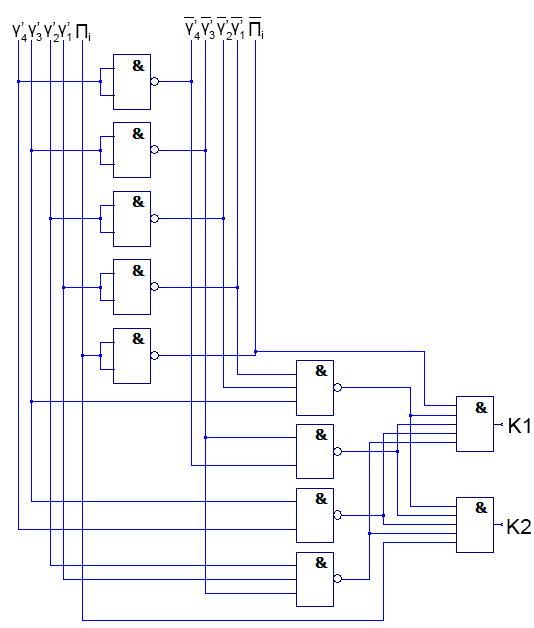
\includegraphics[width=0.5\linewidth]{images/korr_sh_2}
	\caption{Логическая схема корректор}
	\label{fig:korr_sh}
\end{figure}

\subsection{Разработка схемы одноразрядного десятичного сумматора}

Cхемв одноразрядного сумматора будет выглядеть следующим образом:

\begin{figure}[H]
	\centering
	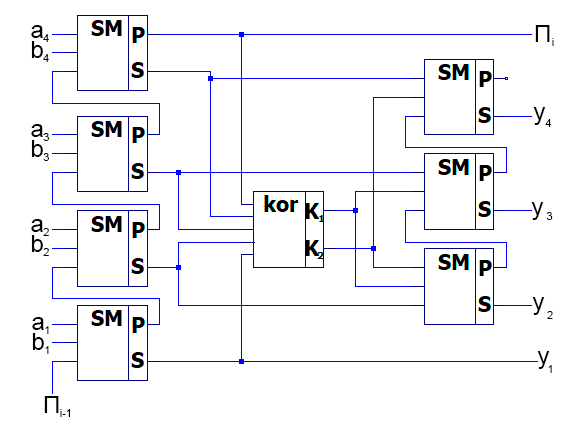
\includegraphics[width=0.5\linewidth]{images/odnSum_sh}
	\caption{Логическая схема одноразрядного сумматора}
	\label{fig:odnSum_sh}
\end{figure}

%В зависимости от результата после пераого этапа сложения может сгенерироватся

В дальнейшем эта схема бует изображаться следующим образом:

\begin{figure}[H]
	\centering
	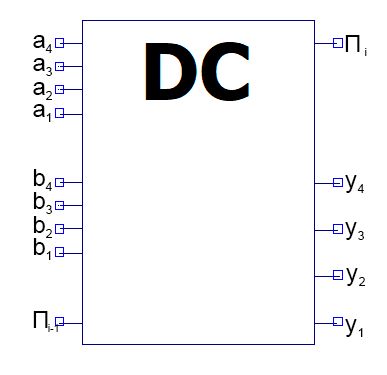
\includegraphics[width=0.2\linewidth]{images/odnSum_el}
	\caption{Одноразрядный сумматор}
	\label{fig:odnSum_el}
\end{figure}

$\alpha_4, \alpha_3, \alpha_2, \alpha_1$ -- перавя тетрада;

$\beta_4, \beta_3, \beta_2, \beta_1$ -- вторая тетрада;

$\Pi_{i-1}$ -- перенос из предыдущего разряда;

$\Pi_i$ -- перенос в следующий разряд.

\section{Разработка дополнительных схем для функционирования многоразрядного десятичного сумматора}

\subsection{Разработка преобразователя прямого кода в обратный для работы с отрицательными величинами}

Составим таблицу истиности для пребразователя из проямого кода в обратный.

\begin{table}[H]
				\begin{center}
		\caption{\label{tab:tabl_preobr} Таблица истиности}
	\begin{tabular}{|c|c|c|c|c|c|c|c|c|}
		\hline
		$a_0$ & $a_4$ & $a_3$ & $a_2$ & $a_1$ & $\hat{a}_4$ & $\hat{a}_3$ & $\hat{a}_2$ & $\hat{a}_1$ \\ \hline
		0  & 0  & 0  & 0  & 0  & 0 & 0 & 0 & 0  \\ \hline
		0  & 0  & 0  & 0  & 1  & 0 & 0 & 0 & 1  \\ \hline
		0  & 0  & 0  & 1  & 0  & 0 & 0 & 1 & 0  \\ \hline
		0  & 0  & 0  & 1  & 1  & 0 & 0 & 1 & 1  \\ \hline
		0  & 0  & 1  & 0  & 0  & 0 & 1 & 0 & 0  \\ \hline
		0  & 0  & 1  & 0  & 1  & x & x & x & x  \\ \hline
		0  & 0  & 1  & 1  & 0  & x & x & x & x  \\ \hline
		0  & 0  & 1  & 1  & 1  & x & x & x & x  \\ \hline
		0  & 1  & 0  & 0  & 0  & x & x & x & x  \\ \hline
		0  & 1  & 0  & 0  & 1  & x & x & x & x  \\ \hline
		0  & 1  & 0  & 1  & 0  & x & x & x & x  \\ \hline
		0  & 1  & 0  & 1  & 1  & 1 & 0 & 1 & 1  \\ \hline
		0  & 1  & 1  & 0  & 0  & 1 & 1 & 0 & 0  \\ \hline
		0  & 1  & 1  & 0  & 1  & 1 & 1 & 0 & 1  \\ \hline
		0  & 1  & 1  & 1  & 0  & 1 & 1 & 1 & 0  \\ \hline
		0  & 1  & 1  & 1  & 1  & 1 & 1 & 1 & 1  \\ \hline
		1  & 0  & 0  & 0  & 0  & 1 & 1 & 1 & 1  \\ \hline
		1  & 0  & 0  & 0  & 1  & 1 & 1 & 1 & 0  \\ \hline
		1  & 0  & 0  & 1  & 0  & 1 & 1 & 0 & 1  \\ \hline
		1  & 0  & 0  & 1  & 1  & 1 & 1 & 0 & 0  \\ \hline
		1  & 0  & 1  & 0  & 0  & 1 & 0 & 1 & 1  \\ \hline
		1  & 0  & 1  & 0  & 1  & x & x & x & x  \\ \hline
		1  & 0  & 1  & 1  & 0  & x & x & x & x  \\ \hline
		1  & 0  & 1  & 1  & 1  & x & x & x & x  \\ \hline
		1  & 1  & 0  & 0  & 0  & x & x & x & x  \\ \hline
		1  & 1  & 0  & 0  & 1  & x & x & x & x  \\ \hline
		1  & 1  & 0  & 1  & 0  & x & x & x & x  \\ \hline
		1  & 1  & 0  & 1  & 1  & 0 & 1 & 0 & 0  \\ \hline
		1  & 1  & 1  & 0  & 0  & 0 & 0 & 1 & 1  \\ \hline
		1  & 1  & 1  & 0  & 1  & 0 & 0 & 1 & 0  \\ \hline
		1  & 1  & 1  & 1  & 0  & 0 & 0 & 0 & 1  \\ \hline
		1  & 1  & 1  & 1  & 1  & 0 & 0 & 0 & 0  \\ \hline
	\end{tabular}
\end{center}
\end{table}

%a4

\begin{table}[H]
			\begin{center}
		\caption{\label{tab:a4_preobr} Диаграмма Вейча для функции $\hat{a}_4$}
	\begin{tabular}{cccccccccc}
		                                                  &                                     \multicolumn{4}{c}{$a_1$}                                     &                                  \multicolumn{4}{c}{$\bar{a}_1$}                                  &                        \\
		                                                  &            \multicolumn{2}{c}{$a_0$}            &         \multicolumn{2}{c}{$\bar{a}_0$}         &            \multicolumn{2}{c}{$a_0$}            &         \multicolumn{2}{c}{$\bar{a}_0$}         &                        \\ \cline{2-9}
		   \multicolumn{1}{c|}{\multirow{2}{*}{$a_4$}}    & \multicolumn{1}{c|}{x} & \multicolumn{1}{c|}{1} & \multicolumn{1}{c|}{}  & \multicolumn{1}{c|}{x} & \multicolumn{1}{c|}{x} & \multicolumn{1}{c|}{1} & \multicolumn{1}{c|}{}  & \multicolumn{1}{c|}{x} &      $\bar{a}_2$       \\ \cline{2-9}
		              \multicolumn{1}{c|}{}               & \multicolumn{1}{c|}{1} & \multicolumn{1}{c|}{1} & \multicolumn{1}{c|}{}  & \multicolumn{1}{c|}{}  & \multicolumn{1}{c|}{x} & \multicolumn{1}{c|}{1} & \multicolumn{1}{c|}{}  & \multicolumn{1}{c|}{x} & \multirow{2}{*}{$a_2$} \\ \cline{2-9}
		\multicolumn{1}{c|}{\multirow{2}{*}{$\bar{a}_4$}} & \multicolumn{1}{c|}{}  & \multicolumn{1}{c|}{x} & \multicolumn{1}{c|}{x} & \multicolumn{1}{c|}{1} & \multicolumn{1}{c|}{}  & \multicolumn{1}{c|}{x} & \multicolumn{1}{c|}{x} & \multicolumn{1}{c|}{1} &                        \\ \cline{2-9}
		              \multicolumn{1}{c|}{}               & \multicolumn{1}{c|}{}  & \multicolumn{1}{c|}{x} & \multicolumn{1}{c|}{x} & \multicolumn{1}{c|}{1} & \multicolumn{1}{c|}{}  & \multicolumn{1}{c|}{}  & \multicolumn{1}{c|}{1} & \multicolumn{1}{c|}{1} &      $\bar{a}_2$       \\ \cline{2-9}
		                                                  &      $\bar{a}_3$       &            \multicolumn{2}{c}{$a_3$}            &         \multicolumn{2}{c}{$\bar{a}_3$}         &            \multicolumn{2}{c}{$a_3$}            &      $\bar{a}_3$       &
	\end{tabular}
\end{center}
\end{table}


$$\overline{\hat{a}_4} = a_4 a_0 + \bar{a}_4\bar{a}_0$$
$$\hat{a}_4 = \overline{a_4 a_0} * \overline{\bar{a}_4\bar{a}_0}$$

%a3

\begin{table}[H]
				\begin{center}
		\caption{\label{tab:a3_preobr} Диаграмма Вейча для функции $\hat{a}_3$}


	\begin{tabular}{cccccccccc}
		& \multicolumn{4}{c}{$a_1$} & \multicolumn{4}{c}{$\bar{a}_1$} &  \\
		& \multicolumn{2}{c}{$a_0$} & \multicolumn{2}{c}{$\bar{a}_0$} & \multicolumn{2}{c}{$a_0$} & \multicolumn{2}{c}{$\bar{a}_0$} &  \\ \cline{2-9}
		\multicolumn{1}{c|}{\multirow{2}{*}{$a_0$}} & \multicolumn{1}{c|}{x} & \multicolumn{1}{c|}{1} & \multicolumn{1}{c|}{} & \multicolumn{1}{c|}{x} & \multicolumn{1}{c|}{x} & \multicolumn{1}{c|}{1} & \multicolumn{1}{c|}{} & \multicolumn{1}{c|}{x} & $\bar{a}_2$ \\ \cline{2-9}
		\multicolumn{1}{c|}{} & \multicolumn{1}{c|}{} & \multicolumn{1}{c|}{1} & \multicolumn{1}{c|}{} & \multicolumn{1}{c|}{1} & \multicolumn{1}{c|}{x} & \multicolumn{1}{c|}{1} & \multicolumn{1}{c|}{} & \multicolumn{1}{c|}{x} & \multirow{2}{*}{$a_3$} \\ \cline{2-9}
		\multicolumn{1}{c|}{\multirow{2}{*}{$\bar{a}_4$}} & \multicolumn{1}{c|}{} & \multicolumn{1}{c|}{x} & \multicolumn{1}{c|}{x} & \multicolumn{1}{c|}{1} & \multicolumn{1}{c|}{} & \multicolumn{1}{c|}{x} & \multicolumn{1}{c|}{x} & \multicolumn{1}{c|}{1} &  \\ \cline{2-9}
		\multicolumn{1}{c|}{} & \multicolumn{1}{c|}{} & \multicolumn{1}{c|}{x} & \multicolumn{1}{c|}{x} & \multicolumn{1}{c|}{1} & \multicolumn{1}{c|}{} & \multicolumn{1}{c|}{1} & \multicolumn{1}{c|}{} & \multicolumn{1}{c|}{1} & $\bar{a}_2$ \\ \cline{2-9}
		& $\bar{a}_3$ & \multicolumn{2}{c}{$a_3$} & \multicolumn{2}{c}{$\bar{a}_3$} & \multicolumn{2}{c}{$a_3$} & $\bar{a}_3$ & 
	\end{tabular}
\end{center}
\end{table}

$$\overline{\hat{a}_3} = a_3 a_0 + \bar{a}_3\bar{a}_0$$
$$\hat{a}_3 = \overline{a_3 a_0} * \overline{\bar{a}_3\bar{a}_0}$$


%a2

\begin{table}[H]
				\begin{center}
		\caption{\label{tab:a2_preobr} Диаграмма Вейча для функции $\hat{a}_2$}

		\begin{tabular}{cccccccccc}
			& \multicolumn{4}{c}{$a_1$} & \multicolumn{4}{c}{$\bar{a}_1$} &  \\
			& \multicolumn{2}{c}{$a_0$} & \multicolumn{2}{c}{$\bar{a}_0$} & \multicolumn{2}{c}{$a_0$} & \multicolumn{2}{c}{$\bar{a}_0$} &  \\ \cline{2-9}
			\multicolumn{1}{c|}{\multirow{2}{*}{$a_0$}} & \multicolumn{1}{c|}{x} & \multicolumn{1}{c|}{} & \multicolumn{1}{c|}{1} & \multicolumn{1}{c|}{x} & \multicolumn{1}{c|}{x} & \multicolumn{1}{c|}{} & \multicolumn{1}{c|}{1} & \multicolumn{1}{c|}{x} & $\bar{a}_2$ \\ \cline{2-9}
			\multicolumn{1}{c|}{} & \multicolumn{1}{c|}{1} & \multicolumn{1}{c|}{1} & \multicolumn{1}{c|}{} & \multicolumn{1}{c|}{} & \multicolumn{1}{c|}{x} & \multicolumn{1}{c|}{1} & \multicolumn{1}{c|}{} & \multicolumn{1}{c|}{x} & \multirow{2}{*}{$a_3$} \\ \cline{2-9}
			\multicolumn{1}{c|}{\multirow{2}{*}{$\bar{a}_4$}} & \multicolumn{1}{c|}{1} & \multicolumn{1}{c|}{x} & \multicolumn{1}{c|}{x} & \multicolumn{1}{c|}{} & \multicolumn{1}{c|}{1} & \multicolumn{1}{c|}{x} & \multicolumn{1}{c|}{x} & \multicolumn{1}{c|}{} &  \\ \cline{2-9}
			\multicolumn{1}{c|}{} & \multicolumn{1}{c|}{} & \multicolumn{1}{c|}{x} & \multicolumn{1}{c|}{x} & \multicolumn{1}{c|}{1} & \multicolumn{1}{c|}{} & \multicolumn{1}{c|}{} & \multicolumn{1}{c|}{1} & \multicolumn{1}{c|}{1} & $\bar{a}_2$ \\ \cline{2-9}
			& $\bar{a}_3$ & \multicolumn{2}{c}{$a_3$} & \multicolumn{2}{c}{$\bar{a}_3$} & \multicolumn{2}{c}{$a_3$} & $\bar{a}_3$ & 
		\end{tabular}

\end{center}
\end{table}

$$\overline{\hat{a}_2} = a_2 a_0 + \bar{a}_2\bar{a}_0$$
$$\hat{a}_2 = \overline{a_2 a_0} * \overline{\bar{a}_2\bar{a}_0}$$


%a1

\begin{table}[H]
				\begin{center}
		\caption{\label{tab:a1_preobr} Диаграмма Вейча для функции $\hat{a}_1$}

		\begin{tabular}{cccccccccc}
			& \multicolumn{4}{c}{$a_1$} & \multicolumn{4}{c}{$\bar{a}_1$} &  \\
			& \multicolumn{2}{c}{$a_0$} & \multicolumn{2}{c}{$\bar{a}_0$} & \multicolumn{2}{c}{$a_0$} & \multicolumn{2}{c}{$\bar{a}_0$} &  \\ \cline{2-9}
			\multicolumn{1}{c|}{\multirow{2}{*}{$a_0$}} & \multicolumn{1}{c|}{x} & \multicolumn{1}{c|}{1} & \multicolumn{1}{c|}{} & \multicolumn{1}{c|}{x} & \multicolumn{1}{c|}{x} & \multicolumn{1}{c|}{} & \multicolumn{1}{c|}{1} & \multicolumn{1}{c|}{x} & $\bar{a}_2$ \\ \cline{2-9}
			\multicolumn{1}{c|}{} & \multicolumn{1}{c|}{1} & \multicolumn{1}{c|}{1} & \multicolumn{1}{c|}{} & \multicolumn{1}{c|}{} & \multicolumn{1}{c|}{x} & \multicolumn{1}{c|}{} & \multicolumn{1}{c|}{1} & \multicolumn{1}{c|}{x} & \multirow{2}{*}{$a_3$} \\ \cline{2-9}
			\multicolumn{1}{c|}{\multirow{2}{*}{$\bar{a}_4$}} & \multicolumn{1}{c|}{1} & \multicolumn{1}{c|}{x} & \multicolumn{1}{c|}{x} & \multicolumn{1}{c|}{} & \multicolumn{1}{c|}{} & \multicolumn{1}{c|}{x} & \multicolumn{1}{c|}{x} & \multicolumn{1}{c|}{1} &  \\ \cline{2-9}
			\multicolumn{1}{c|}{} & \multicolumn{1}{c|}{1} & \multicolumn{1}{c|}{x} & \multicolumn{1}{c|}{x} & \multicolumn{1}{c|}{} & \multicolumn{1}{c|}{} & \multicolumn{1}{c|}{} & \multicolumn{1}{c|}{1} & \multicolumn{1}{c|}{1} & $\bar{a}_2$ \\ \cline{2-9}
			& $\bar{a}_3$ & \multicolumn{2}{c}{$a_3$} & \multicolumn{2}{c}{$\bar{a}_3$} & \multicolumn{2}{c}{$a_3$} & $\bar{a}_3$ & 
		\end{tabular}

\end{center}
\end{table}


$$\overline{\hat{a}_1} = a_1 a_0 + \bar{a}_1\bar{a}_0$$
$$\hat{a}_1 = \overline{a_1 a_0} * \overline{\bar{a}_1\bar{a}_0}$$

\begin{figure}[H]
	\centering
	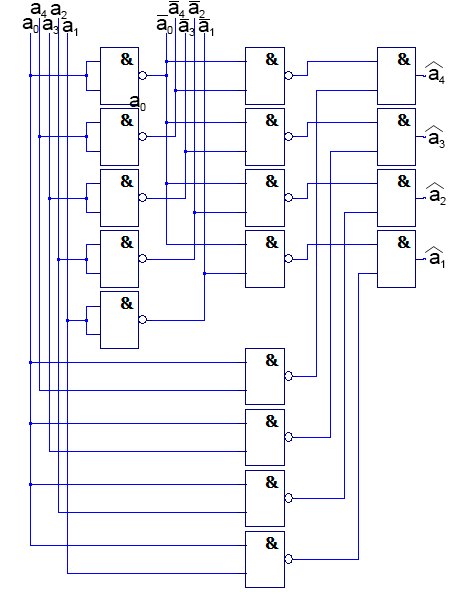
\includegraphics[width=0.5\linewidth]{images/preobr_sh}
	\caption{Логическая схема пребразователя из проямого кода в обратный}
	\label{fig:preobr_sh}
\end{figure}

В дальнейшем эту схему будем обозначать следующим образом:

\begin{figure}[H]
	\centering
	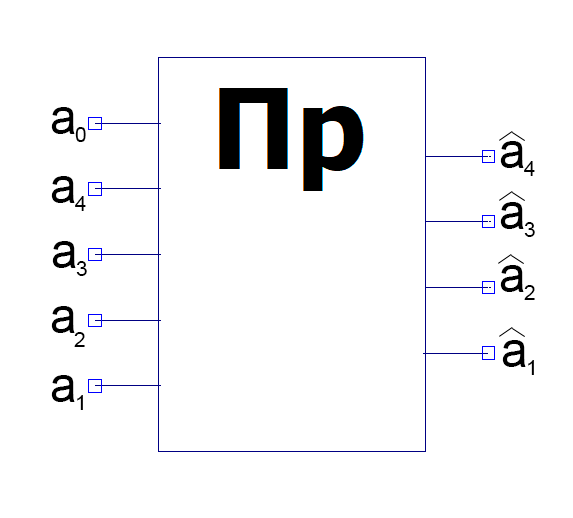
\includegraphics[width=0.3\linewidth]{images/preobr_el}
	\caption{Пребразователь из проямого кода в обратный}
	\label{fig:preobr_el}
\end{figure}

\subsection{Разработка схемы, фиксирующей переполнение разрядной сетки}

Переполнение разрядной сетки происходит, когда:
\begin{itemize}
	\item При сложении двух положительных величин получается отрицательный результат.
	
	\item При сложении двух отрицательных величин получается положительный результат.	
\end{itemize}

\begin{table}[H]
	\begin{center}
		\caption{\label{tab:perSet} Таблица истинности для функции $\varphi$}
		
	\begin{tabular}{|l|l|l|l|}
		\hline
		a0 & b0 & c0 & $\varphi$ \\ \hline
		0  & 0  & 0  & 0  \\ \hline
		0  & 0  & 1  & 1  \\ \hline
		0  & 1  & 0  & 0  \\ \hline
		0  & 1  & 1  & 0  \\ \hline
		1  & 0  & 0  & 0  \\ \hline
		1  & 0  & 1  & 0  \\ \hline
		1  & 1  & 0  & 1  \\ \hline
		1  & 1  & 1  & 0  \\ \hline
	\end{tabular}
\end{center}
\end{table}

\begin{table}[H]
	\begin{center}
		\caption{\label{tab:perSet_ve} Диаграмма Вейча для функции  $\bar{\varphi}$}

\begin{tabular}{ccccc}
	& \multicolumn{2}{c}{$a_0$}                           & \multicolumn{2}{c}{$\bar{a_0}$}                          \\ \cline{2-5} 
	\multicolumn{1}{c|}{$b_0$}  & \multicolumn{1}{c|}{}  & \multicolumn{1}{c|}{1} & \multicolumn{1}{c|}{1} & \multicolumn{1}{c|}{1} \\ \cline{2-5} 
	\multicolumn{1}{c|}{$\bar{b_0}$} & \multicolumn{1}{c|}{1} & \multicolumn{1}{c|}{1} & \multicolumn{1}{c|}{}  & \multicolumn{1}{c|}{1} \\ \cline{2-5} 
	& $\bar{c_0}$                    & \multicolumn{2}{c}{$c_0$}                           & $\bar{c_0}$                   
\end{tabular}
\end{center}
\end{table}

$$\bar\varphi = bc + a\bar{b} + \bar{a}\bar{c}$$

$$\varphi = \overline{bc} *  \overline{a\bar{b}} * \overline{\bar{a}\bar{c}}$$

\begin{figure}[H]
	\centering
	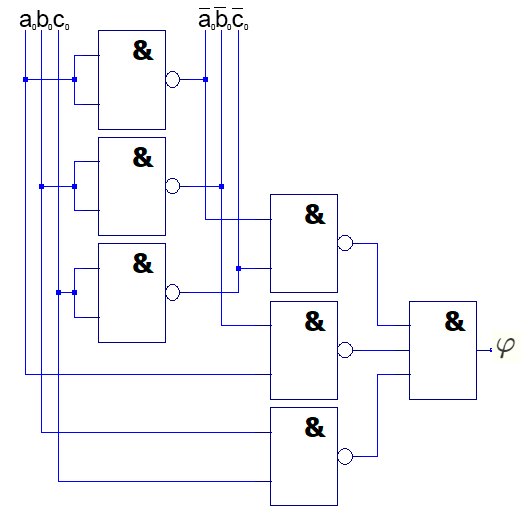
\includegraphics[width=0.5\linewidth]{images/perep_sh}
	\caption{Логическая схема, фиксирующая переполнение разрядной сетки}
	\label{fig:perep_sh}
\end{figure}

В дальнейшем будем обозначать эту схему следующим образом:

\begin{figure}[H]
	\centering
	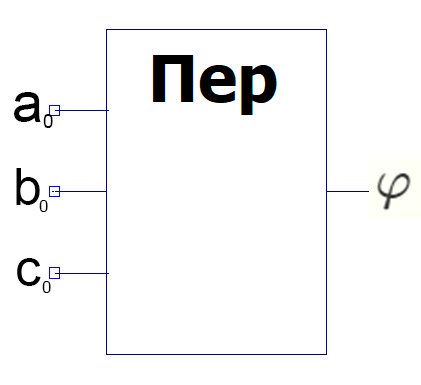
\includegraphics[width=0.2\linewidth]{images/perep_el}
	\caption{Обозначение логической схемы, фиксирующаей переполнение разрядной сетки}
	\label{fig:perep_el}
\end{figure}

\subsection{Разработка схемы для определения знака суммы}

Правило сложения чисел в обратном коде гласит, что при выполнении операции знаковые разряды участвуют в сложении на равне с остальными разрядами. При этом учитывается  переносс взнаковый разряд и перенос из знакового разряда. Поэтому для получения знака результата можно использовать  одноразрядный двоичный сумматор.

\begin{figure}[H]
	\centering
	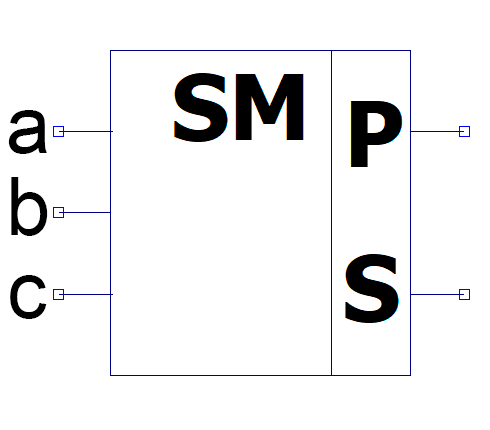
\includegraphics[width=0.2\linewidth]{images/dvSum_el}
	\caption{одноразрядный двоичный сумматор}
	\label{fig:dvSum_el2}
\end{figure}

\section{Разработки функциональной схемы многоразрядного десятичного сумматора}

Обозначим слагаемые на входе сумматора:

\begin{itemize}	
	\item A = a$_0$ a$_1$ a$_2$ a$_3$, где a$_0$ -- знак числа, a$_i$ -- десятичная цифра, которая представляется в двоично-десятичном коде следующим образом:
	a$_i = a^i_4 a^i_3 a^i_2 a^i_1$;
	
	\item B = b$_0$ b$_1$ b$_2$ b$_3$, где b$_0$ -- знак числа, b$_i = \beta^i_4 \beta^i_3 \beta^i_2 \beta^i_1$.	
\end{itemize}

Результат сложения обозначим:
\begin{itemize}	
	\item С = с$_0$ с$_1$ с$_2$ с$_3$, где с$_0$ -- знак числа, с$_i = \gamma^i_4 \gamma^i_3 \gamma^i_2 \gamma^i_1$.	
\end{itemize}

Используя вссе полученные результаты, можно построить структурную схему 3-разрядного десятичного сумматора.

\begin{figure}[H]
	\centering
	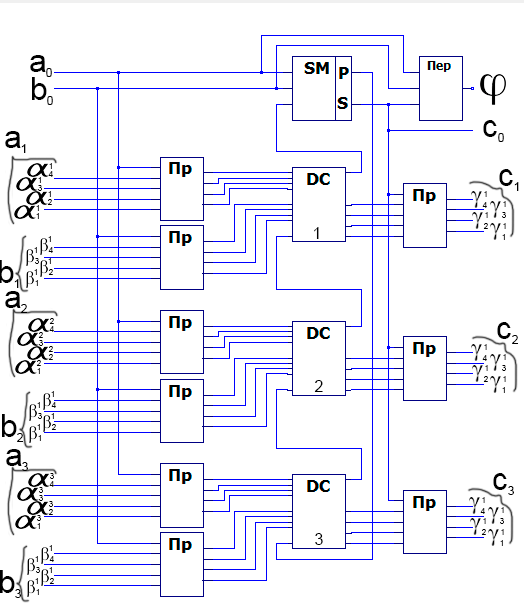
\includegraphics[width=0.5\linewidth]{images/3razrSum}
	\caption{Логическая схема 3-разрядного десятичного сумматора}
	\label{fig:3razrSum}
\end{figure}



\section{Разработка устройства управления для многоразрядного десятичного сумматора}

Для корректной работы устройства в системе должны присутствовать 4 синхроимпульса (СИ1, СИ2, СИ3, СИ4).

\begin{itemize}
	\item СИ1. Первый импульс позволяет записать 2 операнда во входные регистры, сразу после этого величины появляются на входах сумматора и сумматор начинает свою работу;
	
	\item СИ2. Второй импульс записывает в выходной регистр результат суммирования;
	
	\item СИ3. Третий импульс позволяет записать в регистр признаков все признаки результатов;
	
	\item СИ4. Останавливает процесс вычислений.
\end{itemize} 

\subsection{Разработка входных и выходных регистров хранения числовой информации, участвующей в операции сложения}

Регистры входа и выхода имеют одинаковую структуру и строятся на синхронных D-триггерах с асинхронными установочными контактами R и S.
Каждый регистр состоит из 13 триггеров (1 знаковый и 12 знаковых двоичных разрядов).

На вход D подается информационный бит, такой же сигнал и записывается в триггер при поступлении СИ.

\begin{figure}[H]
	\centering
	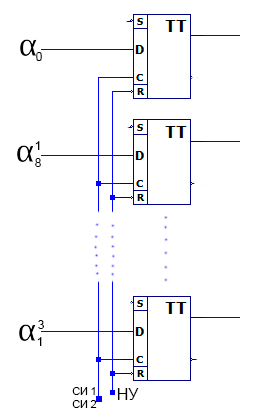
\includegraphics[width=0.4\linewidth]{images/reg}
	\caption{Логическая схема регистров}
	\label{fig:reg}
\end{figure}

\subsection{Разработка регистра признаков результата}

Регистр признаков хранит информацию о результате работы устройства.
Регистр состоит из 4 триггеров.

Первый дает единицу, если результат положительный, второй -- если отрцательный, третий -- если равен нулю, четвертый -- если произошло переполнение (при этом первые 3 триггера блокируются).

\begin{figure}[H]
	\centering
	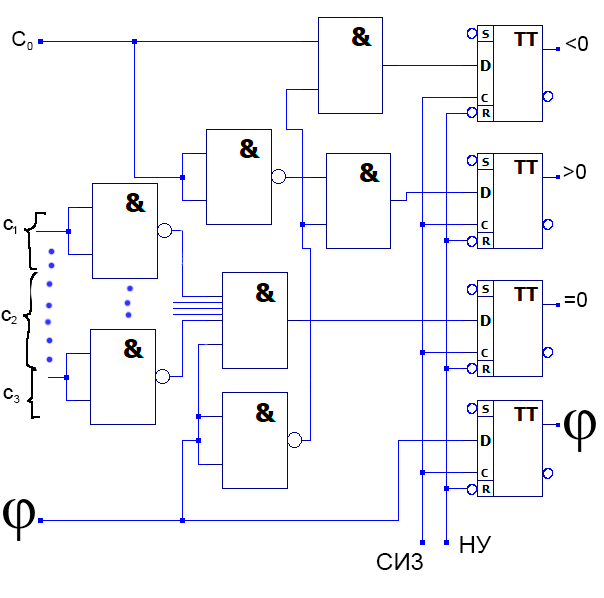
\includegraphics[width=0.5\linewidth]{images/prizn_sh}
	\caption{Логическая схема регистра признаков}
	\label{fig:prizn_sh}
\end{figure}

\subsection{Расчет временных параметров устройства управления}

Определим временные промежутки (Т1, Т2, Т3) между СИ.

Т1 характеризуется длительностью работы трехразрядного деятичного сумматора.
Для определения необходимо определить задеожки сигнплов по каждой схеме, которая входит составной частью в общую схему.

В одноразрядном двоичном сумматоре задержка по цепи вход-выход P равна задержке по цепи вход-выход S и равна $3ns$, это и будет задержкой этого элемента.

Для одноразрядного десятичного сумматора необходимо найти самую длинную цепь. До корректора саммая длинная цепь состоит из трех переносов в следующий разряд и подсчета суммы, итого до корректора $12ns$ ($3ns * 3 + 3ns$).
В следующий разряд ($\Pi_i$) сигнал уйдет через также $12ns$ (цепь из 4 переносов следующй разряд).
Корректор затрчивает $3ns$. Итого, после корректора сумма уже $15ns$.
Далее самая длинная цепочка проходит через 2 переноса в следующий разряд и подсчет суммы.
В сумме одноразрядый десятичный сумматор занимает $24ns$ ($15ns + 3ns * 2 + 3 ns$).

Задержка в пребразователе равна $3ns$.

Схема, фиксирующая переполнение разрядной сетки занимае  $3ns$.

В 3-разрядном десятичном сумматоре самой длиной цепью будет следуюйщая цепь:
\begin{enumerate}
	\item Преобразование -- $3ns$
	\item DC3 перенос в следующий разряд -- $12ns$
	\item DC2 перенос в следующий разряд -- $12ns$
	\item DC1 перенос двоичный сумматор -- $12ns$
	\item Двоичный сумматор -- $3ns$
	\item Одноразрядный десятичный сумматор DC3 -- $24ns$
	\item Преобразование -- $3ns$
\end{enumerate}

Итого, $3 + 12 + 12 + 12 + 3 + 24 + 3 = 69ns$

Так как $T_1$ должно быть кратно 4 (длительность  импульса $2ns$ и промежуток $2ns$), то $T_1 = 72ns$.

$T_2$ определяется задержкой во входных цепях регистра признаков, комбинационная схема на входе триггера имеет задержку не превосходящую $4ns$, значит $T_2 = 4ns$.

Величина $T_3$ также равна $4ns$, так как сигнал останова СИ4 идет непосредственно за сигналом СИ3.

Имея временные интервалы между выходными сигналами в распределителе сигналов, можно приступить к проектированию данного устройства.
Распределитель сигналов является генератором следующих четырехразрядных двоичныхчисел:

$0001,0000 - 17$ раз$, 0010, 0100, 1000$

\subsection{Разработка схемы для получения управляющих сигналов и схемы пуска выполнения операции сложения}

Имея комбинацию выходных сигналов, составим таблицу истинности для генератора сигналов.



\begin{landscape}
\begin{table}[H]
	\begin{center}
		\caption{\label{tab:rasp} Таблица истинности для генератора сигналов}

		\begin{tabular}{|c|c|c|c|c|c|c|c|c|c|c|c|c|c|c|c|c|c|c|}
			\hline
			$Q^5_n$ & $Q^4_n$ & $Q^3_n$ & $Q^2_n$ & $Q^1_n$ & $Q^5_{n+1}$ & $Q^4_{n+1}$ & $Q^3_{n+1}$ & $Q^2_{n+1}$ & $Q^1_{n+1}$ & $F_5$ & $F_4$ & $F_3$ & $F_2$ & $F_1$ & СИ4 & СИ3 & СИ2 & СИ1 \\ \hline
			0 & 0 & 0 & 0 & 0 & 0 & 0 & 0 & 0 & 1 & 0 & 0 & 0 & 0 & $\bigtriangleup$ & 0 & 0 & 0 & 1 \\ \hline
			0 & 0 & 0 & 0 & 1 & 0 & 0 & 0 & 1 & 0 & 0 & 0 & 0 & $\bigtriangleup$ & $\bigtriangledown$ & 0 & 0 & 0 & 0 \\ \hline
			0 & 0 & 0 & 1 & 0 & 0 & 0 & 0 & 1 & 1 & 0 & 0 & 0 & 1 & $\bigtriangleup$ & 0 & 0 & 0 & 0 \\ \hline
			0 & 0 & 0 & 1 & 1 & 0 & 0 & 1 & 0 & 0 & 0 & 0 & $\bigtriangleup$ & $\bigtriangledown$ & $\bigtriangledown$ & 0 & 0 & 0 & 0 \\ \hline
			0 & 0 & 1 & 0 & 0 & 0 & 0 & 1 & 0 & 1 & 0 & 0 & 1 & 0 & $\bigtriangleup$ & 0 & 0 & 0 & 0 \\ \hline
			0 & 0 & 1 & 0 & 1 & 0 & 0 & 1 & 1 & 0 & 0 & 0 & 1 & $\bigtriangleup$ & $\bigtriangledown$ & 0 & 0 & 0 & 0 \\ \hline
			0 & 0 & 1 & 1 & 0 & 0 & 0 & 1 & 1 & 1 & 0 & 0 & 1 & 1 & $\bigtriangleup$ & 0 & 0 & 0 & 0 \\ \hline
			0 & 0 & 1 & 1 & 1 & 0 & 1 & 0 & 0 & 0 & 0 & $\bigtriangleup$ & $\bigtriangledown$ & $\bigtriangledown$ & $\bigtriangledown$ & 0 & 0 & 0 & 0 \\ \hline
			0 & 1 & 0 & 0 & 0 & 0 & 1 & 0 & 0 & 1 & 0 & 1 & 0 & 0 & $\bigtriangleup$ & 0 & 0 & 0 & 0 \\ \hline
			0 & 1 & 0 & 0 & 1 & 0 & 1 & 0 & 1 & 0 & 0 & 1 & 0 & $\bigtriangleup$ & $\bigtriangledown$ & 0 & 0 & 0 & 0 \\ \hline
			0 & 1 & 0 & 1 & 0 & 0 & 1 & 0 & 1 & 1 & 0 & 1 & 0 & 1 & $\bigtriangleup$ & 0 & 0 & 0 & 0 \\ \hline
			0 & 1 & 0 & 1 & 1 & 0 & 1 & 1 & 0 & 0 & 0 & 1 & $\bigtriangleup$ & $\bigtriangledown$ & $\bigtriangledown$ & 0 & 0 & 0 & 0 \\ \hline
			0 & 1 & 1 & 0 & 0 & 0 & 1 & 1 & 0 & 1 & 0 & 1 & 1 & 0 & $\bigtriangleup$ & 0 & 0 & 0 & 0 \\ \hline
			0 & 1 & 1 & 0 & 1 & 0 & 1 & 1 & 1 & 0 & 0 & 1 & 1 & $\bigtriangleup$ & $\bigtriangledown$ & 0 & 0 & 0 & 0 \\ \hline
			0 & 1 & 1 & 1 & 0 & 0 & 1 & 1 & 1 & 1 & 0 & 1 & 1 & 1 & $\bigtriangleup$ & 0 & 0 & 0 & 0 \\ \hline
			0 & 1 & 1 & 1 & 1 & 1 & 0 & 0 & 0 & 1 & $\bigtriangleup$ & $\bigtriangledown$ & $\bigtriangledown$ & $\bigtriangledown$ & $\bigtriangledown$ & 0 & 0 & 0 & 0 \\ \hline
			1 & 0 & 0 & 0 & 1 & 1 & 0 & 0 & 0 & 1 & 1 & 0 & 0 & 0 & $\bigtriangleup$ & 0 & 0 & 0 & 0 \\ \hline
			1 & 0 & 0 & 0 & 1 & 1 & 0 & 0 & 1 & 1 & 1 & 0 & 0 & $\bigtriangleup$ & $\bigtriangledown$ & 0 & 0 & 0 & 0 \\ \hline
			1 & 0 & 0 & 1 & 1 & 1 & 0 & 0 & 1 & 1 & 1 & 0 & 0 & 1 & $\bigtriangleup$ & 0 & 0 & 1 & 0 \\ \hline
			1 & 0 & 0 & 1 & 1 & 1 & 0 & 1 & 0 & 0 & 1 & 0 & $\bigtriangleup$ & $\bigtriangledown$ & $\bigtriangledown$ & 0 & 1 & 0 & 0 \\ \hline
			1 & 0 & 1 & 0 & 0 & 0 & 0 & 0 & 0 & 0 & $\bigtriangledown$ & 0 & $\bigtriangledown$ & 0 & 0 & 1 & 0 & 0 & 0 \\ \hline
		\end{tabular}

\end{center}
\end{table}
\end{landscape}

Составим функции переходов. Так как в работе используются D-триггеры, то по полученным функциям переходов будем находить входные сигналы триггеров.

%F5

\begin{table}[H]
	\begin{center}
		\caption{\label{tab:F5_tab} Диаграмма Вейча для функции переходов $F_5$ }
\begin{tabular}{cccccccccc}
	& \multicolumn{4}{c}{$Q_1$} & \multicolumn{4}{c}{$\bar{Q}_1$} &  \\
	& \multicolumn{2}{c}{$Q_5$} & \multicolumn{2}{c}{$\bar{Q}_5$} & \multicolumn{2}{c}{$Q_5$} & \multicolumn{2}{c}{$\bar{Q}_5$} &  \\ \cline{2-9}
	\multicolumn{1}{c|}{\multirow{2}{*}{$Q_4$}} & \multicolumn{1}{c|}{X} & \multicolumn{1}{c|}{X} & \multicolumn{1}{c|}{} & \multicolumn{1}{c|}{} & \multicolumn{1}{c|}{X} & \multicolumn{1}{c|}{X} & \multicolumn{1}{c|}{} & \multicolumn{1}{c|}{} & $\bar{Q}_2$ \\ \cline{2-9}
	\multicolumn{1}{c|}{} & \multicolumn{1}{c|}{X} & \multicolumn{1}{c|}{X} & \multicolumn{1}{c|}{$\bigtriangleup$} & \multicolumn{1}{c|}{} & \multicolumn{1}{c|}{X} & \multicolumn{1}{c|}{X} & \multicolumn{1}{c|}{} & \multicolumn{1}{c|}{} & \multirow{2}{*}{$Q_2$} \\ \cline{2-9}
	\multicolumn{1}{c|}{\multirow{2}{*}{$\bar{Q}_4$}} & \multicolumn{1}{c|}{1} & \multicolumn{1}{c|}{X} & \multicolumn{1}{c|}{} & \multicolumn{1}{c|}{} & \multicolumn{1}{c|}{1} & \multicolumn{1}{c|}{X} & \multicolumn{1}{c|}{} & \multicolumn{1}{c|}{} &  \\ \cline{2-9}
	\multicolumn{1}{c|}{} & \multicolumn{1}{c|}{1} & \multicolumn{1}{c|}{X} & \multicolumn{1}{c|}{} & \multicolumn{1}{c|}{} & \multicolumn{1}{c|}{1} & \multicolumn{1}{c|}{$\bigtriangledown$} & \multicolumn{1}{c|}{} & \multicolumn{1}{c|}{} & $\bar{Q}_2$ \\ \cline{2-9}
	&  & \multicolumn{2}{c}{} & \multicolumn{2}{c}{} & \multicolumn{2}{c}{} &  &  \\
	& $\bar{Q}_3$ & \multicolumn{2}{c}{$Q_3$} & \multicolumn{2}{c}{$\bar{Q}_3$} & \multicolumn{2}{c}{$Q_3$} & $\bar{Q}_3$ & 
\end{tabular}
\end{center}
\end{table}

%D5

\begin{table}[H]
	\begin{center}
		\caption{\label{tab:D5_tab} Диаграмма Вейча для функции переключения триггера $D_5$ }
		\begin{tabular}{cccccccccc}
			& \multicolumn{4}{c}{$Q_1$} & \multicolumn{4}{c}{$\bar{Q}_1$} &  \\
			& \multicolumn{2}{c}{$Q_5$} & \multicolumn{2}{c}{$\bar{Q}_5$} & \multicolumn{2}{c}{$Q_5$} & \multicolumn{2}{c}{$\bar{Q}_5$} &  \\ \cline{2-9}
			\multicolumn{1}{c|}{\multirow{2}{*}{$Q_4$}} & \multicolumn{1}{c|}{X} & \multicolumn{1}{c|}{X} & \multicolumn{1}{c|}{} & \multicolumn{1}{c|}{} & \multicolumn{1}{c|}{X} & \multicolumn{1}{c|}{X} & \multicolumn{1}{c|}{} & \multicolumn{1}{c|}{} & $\bar{Q}_2$ \\ \cline{2-9}
			\multicolumn{1}{c|}{} & \multicolumn{1}{c|}{X} & \multicolumn{1}{c|}{X} & \multicolumn{1}{c|}{$\bigtriangleup$} & \multicolumn{1}{c|}{} & \multicolumn{1}{c|}{X} & \multicolumn{1}{c|}{X} & \multicolumn{1}{c|}{} & \multicolumn{1}{c|}{} & \multirow{2}{*}{$Q_2$} \\ \cline{2-9}
			\multicolumn{1}{c|}{\multirow{2}{*}{$\bar{Q}_4$}} & \multicolumn{1}{c|}{1} & \multicolumn{1}{c|}{X} & \multicolumn{1}{c|}{} & \multicolumn{1}{c|}{} & \multicolumn{1}{c|}{1} & \multicolumn{1}{c|}{X} & \multicolumn{1}{c|}{} & \multicolumn{1}{c|}{} &  \\ \cline{2-9}
			\multicolumn{1}{c|}{} & \multicolumn{1}{c|}{1} & \multicolumn{1}{c|}{X} & \multicolumn{1}{c|}{} & \multicolumn{1}{c|}{} & \multicolumn{1}{c|}{1} & \multicolumn{1}{c|}{$\bigtriangledown$} & \multicolumn{1}{c|}{} & \multicolumn{1}{c|}{} & $\bar{Q}_2$ \\ \cline{2-9}
			&  & \multicolumn{2}{c}{} & \multicolumn{2}{c}{} & \multicolumn{2}{c}{} &  &  \\
			& $\bar{Q}_3$ & \multicolumn{2}{c}{$Q_3$} & \multicolumn{2}{c}{$\bar{Q}_3$} & \multicolumn{2}{c}{$Q_3$} & $\bar{Q}_3$ & 
		\end{tabular}
	\end{center}
\end{table}

%-D5

\begin{table}[H]
	\begin{center}
		\caption{\label{tab:unD5_tab} Диаграмма Вейча для функции переключения триггера $\overline{D}_5$ }
\begin{tabular}{cccccccccc}
	& \multicolumn{4}{c}{$Q_1$} & \multicolumn{4}{c}{$\bar{Q}_1$} &  \\
	& \multicolumn{2}{c}{$Q_5$} & \multicolumn{2}{c}{$\bar{Q}_5$} & \multicolumn{2}{c}{$Q_5$} & \multicolumn{2}{c}{$\bar{Q}_5$} &  \\ \cline{2-9}
	\multicolumn{1}{c|}{\multirow{2}{*}{$Q_4$}} & \multicolumn{1}{c|}{X} & \multicolumn{1}{c|}{X} & \multicolumn{1}{c|}{1} & \multicolumn{1}{c|}{1} & \multicolumn{1}{c|}{X} & \multicolumn{1}{c|}{X} & \multicolumn{1}{c|}{1} & \multicolumn{1}{c|}{1} & $\bar{Q}_2$ \\ \cline{2-9}
	\multicolumn{1}{c|}{} & \multicolumn{1}{c|}{X} & \multicolumn{1}{c|}{X} & \multicolumn{1}{c|}{} & \multicolumn{1}{c|}{1} & \multicolumn{1}{c|}{X} & \multicolumn{1}{c|}{X} & \multicolumn{1}{c|}{1} & \multicolumn{1}{c|}{1} & \multirow{2}{*}{$Q_2$} \\ \cline{2-9}
	\multicolumn{1}{c|}{\multirow{2}{*}{$\bar{Q}_4$}} & \multicolumn{1}{c|}{} & \multicolumn{1}{c|}{X} & \multicolumn{1}{c|}{1} & \multicolumn{1}{c|}{1} & \multicolumn{1}{c|}{} & \multicolumn{1}{c|}{X} & \multicolumn{1}{c|}{1} & \multicolumn{1}{c|}{1} &  \\ \cline{2-9}
	\multicolumn{1}{c|}{} & \multicolumn{1}{c|}{} & \multicolumn{1}{c|}{X} & \multicolumn{1}{c|}{1} & \multicolumn{1}{c|}{1} & \multicolumn{1}{c|}{} & \multicolumn{1}{c|}{1} & \multicolumn{1}{c|}{1} & \multicolumn{1}{c|}{1} & $\bar{Q}_2$ \\ \cline{2-9}
	&  & \multicolumn{2}{c}{} & \multicolumn{2}{c}{} & \multicolumn{2}{c}{} &  &  \\
	& $\bar{Q}_3$ & \multicolumn{2}{c}{$Q_3$} & \multicolumn{2}{c}{$\bar{Q}_3$} & \multicolumn{2}{c}{$Q_3$} & $\bar{Q}_3$ & 
\end{tabular}
	\end{center}
\end{table}

$$\overline{D}_5 = Q_4\overline{Q}_2 + \overline{Q}_3\overline{Q}_5 + \overline{Q}_3\overline{Q}_4 + Q_4\overline{Q}_1$$

$$D_5 = \overline{Q_4\overline{Q}_2} * \overline{\overline{Q}_3\overline{Q}_5} * \overline{\overline{Q}_3\overline{Q}_4} * \overline{Q_4\overline{Q}_1}$$


%F4

\begin{table}[H]
	\begin{center}
		\caption{\label{tab:F4_tab} Диаграмма Вейча для функции переходов $F_4$ }
\begin{tabular}{cccccccccc}
	& \multicolumn{4}{c}{$Q_1$} & \multicolumn{4}{c}{$\bar{Q}_1$} &  \\
	& \multicolumn{2}{c}{$Q_5$} & \multicolumn{2}{c}{$\bar{Q}_5$} & \multicolumn{2}{c}{$Q_5$} & \multicolumn{2}{c}{$\bar{Q}_5$} &  \\ \cline{2-9}
	\multicolumn{1}{c|}{\multirow{2}{*}{$Q_4$}} & \multicolumn{1}{c|}{X} & \multicolumn{1}{c|}{X} & \multicolumn{1}{c|}{1} & \multicolumn{1}{c|}{1} & \multicolumn{1}{c|}{X} & \multicolumn{1}{c|}{X} & \multicolumn{1}{c|}{1} & \multicolumn{1}{c|}{1} & $\bar{Q}_2$ \\ \cline{2-9}
	\multicolumn{1}{c|}{} & \multicolumn{1}{c|}{X} & \multicolumn{1}{c|}{X} & \multicolumn{1}{c|}{$\bigtriangledown$} & \multicolumn{1}{c|}{1} & \multicolumn{1}{c|}{X} & \multicolumn{1}{c|}{X} & \multicolumn{1}{c|}{1} & \multicolumn{1}{c|}{1} & \multirow{2}{*}{$Q_2$} \\ \cline{2-9}
	\multicolumn{1}{c|}{\multirow{2}{*}{$\bar{Q}_4$}} & \multicolumn{1}{c|}{} & \multicolumn{1}{c|}{X} & \multicolumn{1}{c|}{$\bigtriangleup$} & \multicolumn{1}{c|}{} & \multicolumn{1}{c|}{X} & \multicolumn{1}{c|}{} & \multicolumn{1}{c|}{} & \multicolumn{1}{c|}{1} &  \\ \cline{2-9}
	\multicolumn{1}{c|}{} & \multicolumn{1}{c|}{} & \multicolumn{1}{c|}{X} & \multicolumn{1}{c|}{} & \multicolumn{1}{c|}{} & \multicolumn{1}{c|}{} & \multicolumn{1}{c|}{} & \multicolumn{1}{c|}{} & \multicolumn{1}{c|}{} & $\bar{Q}_2$ \\ \cline{2-9}
	&  & \multicolumn{2}{c}{} & \multicolumn{2}{c}{} & \multicolumn{2}{c}{} &  &  \\
	& $\bar{Q}_3$ & \multicolumn{2}{c}{$Q_3$} & \multicolumn{2}{c}{$\bar{Q}_3$} & \multicolumn{2}{c}{$Q_3$} & $\bar{Q}_3$ & 
\end{tabular}
	\end{center}
\end{table}

%D4

\begin{table}[H]
	\begin{center}
		\caption{\label{tab:D4_tab} Диаграмма Вейча для функции переключения триггера $D_4$ }
		\begin{tabular}{cccccccccc}
			& \multicolumn{4}{c}{$Q_1$} & \multicolumn{4}{c}{$\bar{Q}_1$} &  \\
			& \multicolumn{2}{c}{$Q_5$} & \multicolumn{2}{c}{$\bar{Q}_5$} & \multicolumn{2}{c}{$Q_5$} & \multicolumn{2}{c}{$\bar{Q}_5$} &  \\ \cline{2-9}
			\multicolumn{1}{c|}{\multirow{2}{*}{$Q_4$}} & \multicolumn{1}{c|}{X} & \multicolumn{1}{c|}{X} & \multicolumn{1}{c|}{1} & \multicolumn{1}{c|}{1} & \multicolumn{1}{c|}{X} & \multicolumn{1}{c|}{X} & \multicolumn{1}{c|}{1} & \multicolumn{1}{c|}{1} & $\bar{Q}_2$ \\ \cline{2-9}
			\multicolumn{1}{c|}{} & \multicolumn{1}{c|}{X} & \multicolumn{1}{c|}{X} & \multicolumn{1}{c|}{} & \multicolumn{1}{c|}{1} & \multicolumn{1}{c|}{X} & \multicolumn{1}{c|}{X} & \multicolumn{1}{c|}{1} & \multicolumn{1}{c|}{1} & \multirow{2}{*}{$Q_2$} \\ \cline{2-9}
			\multicolumn{1}{c|}{\multirow{2}{*}{$\bar{Q}_4$}} & \multicolumn{1}{c|}{} & \multicolumn{1}{c|}{X} & \multicolumn{1}{c|}{1} & \multicolumn{1}{c|}{} & \multicolumn{1}{c|}{} & \multicolumn{1}{c|}{X} & \multicolumn{1}{c|}{} & \multicolumn{1}{c|}{} &  \\ \cline{2-9}
			\multicolumn{1}{c|}{} & \multicolumn{1}{c|}{} & \multicolumn{1}{c|}{X} & \multicolumn{1}{c|}{} & \multicolumn{1}{c|}{} & \multicolumn{1}{c|}{} & \multicolumn{1}{c|}{} & \multicolumn{1}{c|}{} & \multicolumn{1}{c|}{} & $\bar{Q}_2$ \\ \cline{2-9}
			&  & \multicolumn{2}{c}{} & \multicolumn{2}{c}{} & \multicolumn{2}{c}{} &  &  \\
			& $\bar{Q}_3$ & \multicolumn{2}{c}{$Q_3$} & \multicolumn{2}{c}{$\bar{Q}_3$} & \multicolumn{2}{c}{$Q_3$} & $\bar{Q}_3$ & 
		\end{tabular}
	\end{center}
\end{table}

%-D4

\begin{table}[H]
	\begin{center}
		\caption{\label{tab:unD4_tab} Диаграмма Вейча для функции переключения триггера $\overline{D}_4$ }
		\begin{tabular}{cccccccccc}
			& \multicolumn{4}{c}{$Q_1$} & \multicolumn{4}{c}{$\bar{Q}_1$} &  \\
			& \multicolumn{2}{c}{$Q_5$} & \multicolumn{2}{c}{$\bar{Q}_5$} & \multicolumn{2}{c}{$Q_5$} & \multicolumn{2}{c}{$\bar{Q}_5$} &  \\ \cline{2-9}
			\multicolumn{1}{c|}{\multirow{2}{*}{$Q_4$}} & \multicolumn{1}{c|}{X} & \multicolumn{1}{c|}{X} & \multicolumn{1}{c|}{} & \multicolumn{1}{c|}{} & \multicolumn{1}{c|}{X} & \multicolumn{1}{c|}{X} & \multicolumn{1}{c|}{} & \multicolumn{1}{c|}{} & $\bar{Q}_2$ \\ \cline{2-9}
			\multicolumn{1}{c|}{} & \multicolumn{1}{c|}{X} & \multicolumn{1}{c|}{X} & \multicolumn{1}{c|}{1} & \multicolumn{1}{c|}{} & \multicolumn{1}{c|}{X} & \multicolumn{1}{c|}{X} & \multicolumn{1}{c|}{} & \multicolumn{1}{c|}{} & \multirow{2}{*}{$Q_2$} \\ \cline{2-9}
			\multicolumn{1}{c|}{\multirow{2}{*}{$\bar{Q}_4$}} & \multicolumn{1}{c|}{1} & \multicolumn{1}{c|}{X} & \multicolumn{1}{c|}{} & \multicolumn{1}{c|}{1} & \multicolumn{1}{c|}{1} & \multicolumn{1}{c|}{X} & \multicolumn{1}{c|}{1} & \multicolumn{1}{c|}{1} &  \\ \cline{2-9}
			\multicolumn{1}{c|}{} & \multicolumn{1}{c|}{1} & \multicolumn{1}{c|}{X} & \multicolumn{1}{c|}{1} & \multicolumn{1}{c|}{1} & \multicolumn{1}{c|}{1} & \multicolumn{1}{c|}{1} & \multicolumn{1}{c|}{1} & \multicolumn{1}{c|}{1} & $\bar{Q}_2$ \\ \cline{2-9}
			&  & \multicolumn{2}{c}{} & \multicolumn{2}{c}{} & \multicolumn{2}{c}{} &  &  \\
			& $\bar{Q}_3$ & \multicolumn{2}{c}{$Q_3$} & \multicolumn{2}{c}{$\bar{Q}_3$} & \multicolumn{2}{c}{$Q_3$} & $\bar{Q}_3$ & 
		\end{tabular}
	\end{center}
\end{table}

$$\overline{D}_4 = Q_4Q_3Q_2Q_1 + \overline{Q}_4\overline{Q}_3 + \overline{Q}_4\overline{Q}_2 + \overline{Q}_4\overline{Q}_1$$

$$D_4 = \overline{Q_4Q_3Q_2Q_1} * \overline{\overline{Q}_4\overline{Q}_3}* \overline{\overline{Q}_4\overline{Q}_2}* \overline{\overline{Q}_4\overline{Q}_1}$$


%F3

\begin{table}[H]
	\begin{center}
		\caption{\label{tab:F3_tab} Диаграмма Вейча для функции переходов $F_3$ }
		\begin{tabular}{cccccccccc}
			& \multicolumn{4}{c}{$Q_1$} & \multicolumn{4}{c}{$\bar{Q}_1$} &  \\
			& \multicolumn{2}{c}{$Q_5$} & \multicolumn{2}{c}{$\bar{Q}_5$} & \multicolumn{2}{c}{$Q_5$} & \multicolumn{2}{c}{$\bar{Q}_5$} &  \\ \cline{2-9}
			\multicolumn{1}{c|}{\multirow{2}{*}{$Q_4$}} & \multicolumn{1}{c|}{X} & \multicolumn{1}{c|}{X} & \multicolumn{1}{c|}{1} & \multicolumn{1}{c|}{} & \multicolumn{1}{c|}{X} & \multicolumn{1}{c|}{X} & \multicolumn{1}{c|}{1} & \multicolumn{1}{c|}{} & $\bar{Q}_2$ \\ \cline{2-9}
			\multicolumn{1}{c|}{} & \multicolumn{1}{c|}{X} & \multicolumn{1}{c|}{X} & \multicolumn{1}{c|}{$\bigtriangledown$} & \multicolumn{1}{c|}{$\bigtriangleup$} & \multicolumn{1}{c|}{X} & \multicolumn{1}{c|}{X} & \multicolumn{1}{c|}{1} & \multicolumn{1}{c|}{} & \multirow{2}{*}{$Q_2$} \\ \cline{2-9}
			\multicolumn{1}{c|}{\multirow{2}{*}{$\bar{Q}_4$}} & \multicolumn{1}{c|}{$\bigtriangleup$} & \multicolumn{1}{c|}{X} & \multicolumn{1}{c|}{$\bigtriangledown$} & \multicolumn{1}{c|}{$\bigtriangleup$} & \multicolumn{1}{c|}{} & \multicolumn{1}{c|}{X} & \multicolumn{1}{c|}{1} & \multicolumn{1}{c|}{} &  \\ \cline{2-9}
			\multicolumn{1}{c|}{} & \multicolumn{1}{c|}{} & \multicolumn{1}{c|}{X} & \multicolumn{1}{c|}{1} & \multicolumn{1}{c|}{} & \multicolumn{1}{c|}{} & \multicolumn{1}{c|}{$\bigtriangledown$} & \multicolumn{1}{c|}{1} & \multicolumn{1}{c|}{} & $\bar{Q}_2$ \\ \cline{2-9}
			&  & \multicolumn{2}{c}{} & \multicolumn{2}{c}{} & \multicolumn{2}{c}{} &  &  \\
			& $\bar{Q}_3$ & \multicolumn{2}{c}{$Q_3$} & \multicolumn{2}{c}{$\bar{Q}_3$} & \multicolumn{2}{c}{$Q_3$} & $\bar{Q}_3$ & 
		\end{tabular}
	\end{center}
\end{table}

%D3

\begin{table}[H]
	\begin{center}
		\caption{\label{tab:D3_tab} Диаграмма Вейча для функции переключения триггера $D_3$ }
		\begin{tabular}{cccccccccc}
			& \multicolumn{4}{c}{$Q_1$} & \multicolumn{4}{c}{$\bar{Q}_1$} &  \\
			& \multicolumn{2}{c}{$Q_5$} & \multicolumn{2}{c}{$\bar{Q}_5$} & \multicolumn{2}{c}{$Q_5$} & \multicolumn{2}{c}{$\bar{Q}_5$} &  \\ \cline{2-9}
			\multicolumn{1}{c|}{\multirow{2}{*}{$Q_4$}} & \multicolumn{1}{c|}{X} & \multicolumn{1}{c|}{X} & \multicolumn{1}{c|}{1} & \multicolumn{1}{c|}{} & \multicolumn{1}{c|}{X} & \multicolumn{1}{c|}{X} & \multicolumn{1}{c|}{1} & \multicolumn{1}{c|}{} & $\bar{Q}_2$ \\ \cline{2-9}
			\multicolumn{1}{c|}{} & \multicolumn{1}{c|}{X} & \multicolumn{1}{c|}{X} & \multicolumn{1}{c|}{} & \multicolumn{1}{c|}{1} & \multicolumn{1}{c|}{X} & \multicolumn{1}{c|}{X} & \multicolumn{1}{c|}{1} & \multicolumn{1}{c|}{} & \multirow{2}{*}{$Q_2$} \\ \cline{2-9}
			\multicolumn{1}{c|}{\multirow{2}{*}{$\bar{Q}_4$}} & \multicolumn{1}{c|}{1} & \multicolumn{1}{c|}{X} & \multicolumn{1}{c|}{} & \multicolumn{1}{c|}{1} & \multicolumn{1}{c|}{} & \multicolumn{1}{c|}{X} & \multicolumn{1}{c|}{1} & \multicolumn{1}{c|}{} &  \\ \cline{2-9}
			\multicolumn{1}{c|}{} & \multicolumn{1}{c|}{} & \multicolumn{1}{c|}{X} & \multicolumn{1}{c|}{1} & \multicolumn{1}{c|}{} & \multicolumn{1}{c|}{} & \multicolumn{1}{c|}{} & \multicolumn{1}{c|}{1} & \multicolumn{1}{c|}{} & $\bar{Q}_2$ \\ \cline{2-9}
			&  & \multicolumn{2}{c}{} & \multicolumn{2}{c}{} & \multicolumn{2}{c}{} &  &  \\
			& $\bar{Q}_3$ & \multicolumn{2}{c}{$Q_3$} & \multicolumn{2}{c}{$\bar{Q}_3$} & \multicolumn{2}{c}{$Q_3$} & $\bar{Q}_3$ & 
		\end{tabular}
	\end{center}
\end{table}

%-D3

\begin{table}[H]
	\begin{center}
		\caption{\label{tab:unD3_tab} Диаграмма Вейча для функции переключения триггера $\overline{D}_3$ }
		\begin{tabular}{cccccccccc}
			& \multicolumn{4}{c}{$Q_1$} & \multicolumn{4}{c}{$\bar{Q}_1$} &  \\
			& \multicolumn{2}{c}{$Q_5$} & \multicolumn{2}{c}{$\bar{Q}_5$} & \multicolumn{2}{c}{$Q_5$} & \multicolumn{2}{c}{$\bar{Q}_5$} &  \\ \cline{2-9}
			\multicolumn{1}{c|}{\multirow{2}{*}{$Q_4$}} & \multicolumn{1}{c|}{X} & \multicolumn{1}{c|}{X} & \multicolumn{1}{c|}{} & \multicolumn{1}{c|}{1} & \multicolumn{1}{c|}{X} & \multicolumn{1}{c|}{X} & \multicolumn{1}{c|}{} & \multicolumn{1}{c|}{1} & $\bar{Q}_2$ \\ \cline{2-9}
			\multicolumn{1}{c|}{} & \multicolumn{1}{c|}{X} & \multicolumn{1}{c|}{X} & \multicolumn{1}{c|}{1} & \multicolumn{1}{c|}{} & \multicolumn{1}{c|}{X} & \multicolumn{1}{c|}{X} & \multicolumn{1}{c|}{} & \multicolumn{1}{c|}{1} & \multirow{2}{*}{$Q_2$} \\ \cline{2-9}
			\multicolumn{1}{c|}{\multirow{2}{*}{$\bar{Q}_4$}} & \multicolumn{1}{c|}{} & \multicolumn{1}{c|}{X} & \multicolumn{1}{c|}{1} & \multicolumn{1}{c|}{} & \multicolumn{1}{c|}{1} & \multicolumn{1}{c|}{X} & \multicolumn{1}{c|}{} & \multicolumn{1}{c|}{1} &  \\ \cline{2-9}
			\multicolumn{1}{c|}{} & \multicolumn{1}{c|}{1} & \multicolumn{1}{c|}{X} & \multicolumn{1}{c|}{} & \multicolumn{1}{c|}{1} & \multicolumn{1}{c|}{1} & \multicolumn{1}{c|}{1} & \multicolumn{1}{c|}{} & \multicolumn{1}{c|}{1} & $\bar{Q}_2$ \\ \cline{2-9}
			&  & \multicolumn{2}{c}{} & \multicolumn{2}{c}{} & \multicolumn{2}{c}{} &  &  \\
			& $\bar{Q}_3$ & \multicolumn{2}{c}{$Q_3$} & \multicolumn{2}{c}{$\bar{Q}_3$} & \multicolumn{2}{c}{$Q_3$} & $\bar{Q}_3$ & 
		\end{tabular}
	\end{center}
\end{table}

$$\overline{D}_3 = Q_3Q_2Q_1 + \overline{Q}_3\overline{Q}_2 + Q_5\overline{Q}_1 + \overline{Q}_3\overline{Q}_1$$

$$D_3 = \overline{Q_3Q_2Q_1} *\overline{\overline{Q}_3\overline{Q}_2} * \overline{Q_5\overline{Q}_1} * \overline{\overline{Q}_3\overline{Q}_1}$$


%F2

\begin{table}[H]
	\begin{center}
		\caption{\label{tab:F2_tab} Диаграмма Вейча для функции переходов $F_2$ }
		\begin{tabular}{cccccccccc}
			& \multicolumn{4}{c}{$Q_1$} & \multicolumn{4}{c}{$\bar{Q}_1$} &  \\
			& \multicolumn{2}{c}{$Q_5$} & \multicolumn{2}{c}{$\bar{Q}_5$} & \multicolumn{2}{c}{$Q_5$} & \multicolumn{2}{c}{$\bar{Q}_5$} &  \\ \cline{2-9}
			\multicolumn{1}{c|}{\multirow{2}{*}{$Q_4$}} & \multicolumn{1}{c|}{X} & \multicolumn{1}{c|}{X} & \multicolumn{1}{c|}{$\bigtriangleup$} & \multicolumn{1}{c|}{$\bigtriangleup$} & \multicolumn{1}{c|}{X} & \multicolumn{1}{c|}{X} & \multicolumn{1}{c|}{} & \multicolumn{1}{c|}{} & $\bar{Q}_2$ \\ \cline{2-9}
			\multicolumn{1}{c|}{} & \multicolumn{1}{c|}{X} & \multicolumn{1}{c|}{X} & \multicolumn{1}{c|}{$\bigtriangledown$} & \multicolumn{1}{c|}{$\bigtriangledown$} & \multicolumn{1}{c|}{X} & \multicolumn{1}{c|}{X} & \multicolumn{1}{c|}{1} & \multicolumn{1}{c|}{1} & \multirow{2}{*}{$Q_2$} \\ \cline{2-9}
			\multicolumn{1}{c|}{\multirow{2}{*}{$\bar{Q}_4$}} & \multicolumn{1}{c|}{$\bigtriangledown$} & \multicolumn{1}{c|}{X} & \multicolumn{1}{c|}{$\bigtriangledown$} & \multicolumn{1}{c|}{$\bigtriangledown$} & \multicolumn{1}{c|}{1} & \multicolumn{1}{c|}{X} & \multicolumn{1}{c|}{1} & \multicolumn{1}{c|}{1} &  \\ \cline{2-9}
			\multicolumn{1}{c|}{} & \multicolumn{1}{c|}{$\bigtriangleup$} & \multicolumn{1}{c|}{X} & \multicolumn{1}{c|}{$\bigtriangleup$} & \multicolumn{1}{c|}{$\bigtriangleup$} & \multicolumn{1}{c|}{} & \multicolumn{1}{c|}{} & \multicolumn{1}{c|}{} & \multicolumn{1}{c|}{} & $\bar{Q}_2$ \\ \cline{2-9}
			&  & \multicolumn{2}{c}{} & \multicolumn{2}{c}{} & \multicolumn{2}{c}{} &  &  \\
			& $\bar{Q}_3$ & \multicolumn{2}{c}{$Q_3$} & \multicolumn{2}{c}{$\bar{Q}_3$} & \multicolumn{2}{c}{$Q_3$} & $\bar{Q}_3$ & 
		\end{tabular}
	\end{center}
\end{table}

%D2

\begin{table}[H]
	\begin{center}
		\caption{\label{tab:D2_tab} Диаграмма Вейча для функции переключения триггера $D_2$ }
		\begin{tabular}{cccccccccc}
			& \multicolumn{4}{c}{$Q_1$} & \multicolumn{4}{c}{$\bar{Q}_1$} &  \\
			& \multicolumn{2}{c}{$Q_5$} & \multicolumn{2}{c}{$\bar{Q}_5$} & \multicolumn{2}{c}{$Q_5$} & \multicolumn{2}{c}{$\bar{Q}_5$} &  \\ \cline{2-9}
			\multicolumn{1}{c|}{\multirow{2}{*}{$Q_4$}} & \multicolumn{1}{c|}{X} & \multicolumn{1}{c|}{X} & \multicolumn{1}{c|}{1} & \multicolumn{1}{c|}{1} & \multicolumn{1}{c|}{X} & \multicolumn{1}{c|}{X} & \multicolumn{1}{c|}{} & \multicolumn{1}{c|}{} & $\bar{Q}_2$ \\ \cline{2-9}
			\multicolumn{1}{c|}{} & \multicolumn{1}{c|}{X} & \multicolumn{1}{c|}{X} & \multicolumn{1}{c|}{} & \multicolumn{1}{c|}{} & \multicolumn{1}{c|}{X} & \multicolumn{1}{c|}{X} & \multicolumn{1}{c|}{1} & \multicolumn{1}{c|}{1} & \multirow{2}{*}{$Q_2$} \\ \cline{2-9}
			\multicolumn{1}{c|}{\multirow{2}{*}{$\bar{Q}_4$}} & \multicolumn{1}{c|}{} & \multicolumn{1}{c|}{X} & \multicolumn{1}{c|}{} & \multicolumn{1}{c|}{} & \multicolumn{1}{c|}{1} & \multicolumn{1}{c|}{X} & \multicolumn{1}{c|}{1} & \multicolumn{1}{c|}{1} &  \\ \cline{2-9}
			\multicolumn{1}{c|}{} & \multicolumn{1}{c|}{1} & \multicolumn{1}{c|}{X} & \multicolumn{1}{c|}{1} & \multicolumn{1}{c|}{1} & \multicolumn{1}{c|}{} & \multicolumn{1}{c|}{} & \multicolumn{1}{c|}{} & \multicolumn{1}{c|}{} & $\bar{Q}_2$ \\ \cline{2-9}
			&  & \multicolumn{2}{c}{} & \multicolumn{2}{c}{} & \multicolumn{2}{c}{} &  &  \\
			& $\bar{Q}_3$ & \multicolumn{2}{c}{$Q_3$} & \multicolumn{2}{c}{$\bar{Q}_3$} & \multicolumn{2}{c}{$Q_3$} & $\bar{Q}_3$ & 
	\end{tabular}
	\end{center}
\end{table}

%-D2

\begin{table}[H]
	\begin{center}
		\caption{\label{tab:unD2_tab} Диаграмма Вейча для функции переключения триггера $\overline{D}_2$ }
	\begin{tabular}{cccccccccc}
		& \multicolumn{4}{c}{$Q_1$} & \multicolumn{4}{c}{$\bar{Q}_1$} &  \\
		& \multicolumn{2}{c}{$Q_5$} & \multicolumn{2}{c}{$\bar{Q}_5$} & \multicolumn{2}{c}{$Q_5$} & \multicolumn{2}{c}{$\bar{Q}_5$} &  \\ \cline{2-9}
		\multicolumn{1}{c|}{\multirow{2}{*}{$Q_4$}} & \multicolumn{1}{c|}{X} & \multicolumn{1}{c|}{X} & \multicolumn{1}{c|}{} & \multicolumn{1}{c|}{} & \multicolumn{1}{c|}{X} & \multicolumn{1}{c|}{X} & \multicolumn{1}{c|}{1} & \multicolumn{1}{c|}{1} & $\bar{Q}_2$ \\ \cline{2-9}
		\multicolumn{1}{c|}{} & \multicolumn{1}{c|}{X} & \multicolumn{1}{c|}{X} & \multicolumn{1}{c|}{1} & \multicolumn{1}{c|}{1} & \multicolumn{1}{c|}{X} & \multicolumn{1}{c|}{X} & \multicolumn{1}{c|}{} & \multicolumn{1}{c|}{} & \multirow{2}{*}{$Q_2$} \\ \cline{2-9}
		\multicolumn{1}{c|}{\multirow{2}{*}{$\bar{Q}_4$}} & \multicolumn{1}{c|}{1} & \multicolumn{1}{c|}{X} & \multicolumn{1}{c|}{1} & \multicolumn{1}{c|}{1} & \multicolumn{1}{c|}{} & \multicolumn{1}{c|}{X} & \multicolumn{1}{c|}{} & \multicolumn{1}{c|}{} &  \\ \cline{2-9}
		\multicolumn{1}{c|}{} & \multicolumn{1}{c|}{} & \multicolumn{1}{c|}{X} & \multicolumn{1}{c|}{} & \multicolumn{1}{c|}{} & \multicolumn{1}{c|}{1} & \multicolumn{1}{c|}{1} & \multicolumn{1}{c|}{1} & \multicolumn{1}{c|}{1} & $\bar{Q}_2$ \\ \cline{2-9}
		&  & \multicolumn{2}{c}{} & \multicolumn{2}{c}{} & \multicolumn{2}{c}{} &  &  \\
		& $\bar{Q}_3$ & \multicolumn{2}{c}{$Q_3$} & \multicolumn{2}{c}{$\bar{Q}_3$} & \multicolumn{2}{c}{$Q_3$} & $\bar{Q}_3$ & 
	\end{tabular}
	\end{center}
\end{table}

$$\overline{D}_2 = Q_2Q_1 + \overline{Q}_3\overline{Q}_2$$

$$D_2 = \overline{Q_2Q_1} * \overline{\overline{Q}_3\overline{Q}_2}$$

%F1

\begin{table}[H]
	\begin{center}
		\caption{\label{tab:F1_tab} Диаграмма Вейча для функции переходов $F_1$ }
		\begin{tabular}{cccccccccc}
			& \multicolumn{4}{c}{$Q_1$} & \multicolumn{4}{c}{$\bar{Q}_1$} &  \\
			& \multicolumn{2}{c}{$Q_5$} & \multicolumn{2}{c}{$\bar{Q}_5$} & \multicolumn{2}{c}{$Q_5$} & \multicolumn{2}{c}{$\bar{Q}_5$} &  \\ \cline{2-9}
			\multicolumn{1}{c|}{\multirow{2}{*}{$Q_4$}} & \multicolumn{1}{c|}{X} & \multicolumn{1}{c|}{X} & \multicolumn{1}{c|}{$\bigtriangledown$} & \multicolumn{1}{c|}{$\bigtriangledown$} & \multicolumn{1}{c|}{X} & \multicolumn{1}{c|}{X} & \multicolumn{1}{c|}{$\bigtriangleup$} & \multicolumn{1}{c|}{$\bigtriangleup$} & $\bar{Q}_2$ \\ \cline{2-9}
			\multicolumn{1}{c|}{} & \multicolumn{1}{c|}{X} & \multicolumn{1}{c|}{X} & \multicolumn{1}{c|}{$\bigtriangledown$} & \multicolumn{1}{c|}{$\bigtriangledown$} & \multicolumn{1}{c|}{X} & \multicolumn{1}{c|}{X} & \multicolumn{1}{c|}{$\bigtriangleup$} & \multicolumn{1}{c|}{$\bigtriangleup$} & \multirow{2}{*}{$Q_2$} \\ \cline{2-9}
			\multicolumn{1}{c|}{\multirow{2}{*}{$\bar{Q}_4$}} & \multicolumn{1}{c|}{$\bigtriangledown$} & \multicolumn{1}{c|}{X} & \multicolumn{1}{c|}{$\bigtriangledown$} & \multicolumn{1}{c|}{$\bigtriangledown$} & \multicolumn{1}{c|}{$\bigtriangleup$} & \multicolumn{1}{c|}{X} & \multicolumn{1}{c|}{$\bigtriangleup$} & \multicolumn{1}{c|}{$\bigtriangleup$} &  \\ \cline{2-9}
			\multicolumn{1}{c|}{} & \multicolumn{1}{c|}{$\bigtriangledown$} & \multicolumn{1}{c|}{X} & \multicolumn{1}{c|}{$\bigtriangledown$} & \multicolumn{1}{c|}{$\bigtriangledown$} & \multicolumn{1}{c|}{$\bigtriangleup$} & \multicolumn{1}{c|}{$\bigtriangleup$} & \multicolumn{1}{c|}{$\bigtriangleup$} & \multicolumn{1}{c|}{1} & $\bar{Q}_2$ \\ \cline{2-9}
			&  & \multicolumn{2}{c}{} & \multicolumn{2}{c}{} & \multicolumn{2}{c}{} &  &  \\
			& $\bar{Q}_3$ & \multicolumn{2}{c}{$Q_3$} & \multicolumn{2}{c}{$\bar{Q}_3$} & \multicolumn{2}{c}{$Q_3$} & $\bar{Q}_3$ & 
		\end{tabular}
	\end{center}
\end{table}

%D1

\begin{table}[H]
	\begin{center}
		\caption{\label{tab:D1_tab} Диаграмма Вейча для функции переключения триггера $D_1$ }
		\begin{tabular}{cccccccccc}
			& \multicolumn{4}{c}{$Q_1$} & \multicolumn{4}{c}{$\bar{Q}_1$} &  \\
			& \multicolumn{2}{c}{$Q_5$} & \multicolumn{2}{c}{$\bar{Q}_5$} & \multicolumn{2}{c}{$Q_5$} & \multicolumn{2}{c}{$\bar{Q}_5$} &  \\ \cline{2-9}
			\multicolumn{1}{c|}{\multirow{2}{*}{$Q_4$}} & \multicolumn{1}{c|}{X} & \multicolumn{1}{c|}{X} & \multicolumn{1}{c|}{} & \multicolumn{1}{c|}{} & \multicolumn{1}{c|}{X} & \multicolumn{1}{c|}{X} & \multicolumn{1}{c|}{1} & \multicolumn{1}{c|}{1} & $\bar{Q}_2$ \\ \cline{2-9}
			\multicolumn{1}{c|}{} & \multicolumn{1}{c|}{X} & \multicolumn{1}{c|}{X} & \multicolumn{1}{c|}{} & \multicolumn{1}{c|}{} & \multicolumn{1}{c|}{X} & \multicolumn{1}{c|}{X} & \multicolumn{1}{c|}{1} & \multicolumn{1}{c|}{1} & \multirow{2}{*}{$Q_2$} \\ \cline{2-9}
			\multicolumn{1}{c|}{\multirow{2}{*}{$\bar{Q}_4$}} & \multicolumn{1}{c|}{} & \multicolumn{1}{c|}{X} & \multicolumn{1}{c|}{} & \multicolumn{1}{c|}{} & \multicolumn{1}{c|}{1} & \multicolumn{1}{c|}{X} & \multicolumn{1}{c|}{1} & \multicolumn{1}{c|}{1} &  \\ \cline{2-9}
			\multicolumn{1}{c|}{} & \multicolumn{1}{c|}{} & \multicolumn{1}{c|}{X} & \multicolumn{1}{c|}{} & \multicolumn{1}{c|}{} & \multicolumn{1}{c|}{1} & \multicolumn{1}{c|}{} & \multicolumn{1}{c|}{1} & \multicolumn{1}{c|}{1} & $\bar{Q}_2$ \\ \cline{2-9}
			&  & \multicolumn{2}{c}{} & \multicolumn{2}{c}{} & \multicolumn{2}{c}{} &  &  \\
			& $\bar{Q}_3$ & \multicolumn{2}{c}{$Q_3$} & \multicolumn{2}{c}{$\bar{Q}_3$} & \multicolumn{2}{c}{$Q_3$} & $\bar{Q}_3$ & 
		\end{tabular}
	\end{center}
\end{table}

%-D1

\begin{table}[H]
	\begin{center}
		\caption{\label{tab:unD1_tab} Диаграмма Вейча для функции переключения триггера $\overline{D}_1$ }
	\begin{tabular}{cccccccccc}
		& \multicolumn{4}{c}{$Q_1$} & \multicolumn{4}{c}{$\bar{Q}_1$} &  \\
		& \multicolumn{2}{c}{$Q_5$} & \multicolumn{2}{c}{$\bar{Q}_5$} & \multicolumn{2}{c}{$Q_5$} & \multicolumn{2}{c}{$\bar{Q}_5$} &  \\ \cline{2-9}
		\multicolumn{1}{c|}{\multirow{2}{*}{$Q_4$}} & \multicolumn{1}{c|}{X} & \multicolumn{1}{c|}{X} & \multicolumn{1}{c|}{1} & \multicolumn{1}{c|}{1} & \multicolumn{1}{c|}{X} & \multicolumn{1}{c|}{X} & \multicolumn{1}{c|}{} & \multicolumn{1}{c|}{} & $\bar{Q}_2$ \\ \cline{2-9}
		\multicolumn{1}{c|}{} & \multicolumn{1}{c|}{X} & \multicolumn{1}{c|}{X} & \multicolumn{1}{c|}{1} & \multicolumn{1}{c|}{1} & \multicolumn{1}{c|}{X} & \multicolumn{1}{c|}{X} & \multicolumn{1}{c|}{} & \multicolumn{1}{c|}{} & \multirow{2}{*}{$Q_2$} \\ \cline{2-9}
		\multicolumn{1}{c|}{\multirow{2}{*}{$\bar{Q}_4$}} & \multicolumn{1}{c|}{1} & \multicolumn{1}{c|}{X} & \multicolumn{1}{c|}{1} & \multicolumn{1}{c|}{1} & \multicolumn{1}{c|}{} & \multicolumn{1}{c|}{X} & \multicolumn{1}{c|}{} & \multicolumn{1}{c|}{} &  \\ \cline{2-9}
		\multicolumn{1}{c|}{} & \multicolumn{1}{c|}{1} & \multicolumn{1}{c|}{X} & \multicolumn{1}{c|}{1} & \multicolumn{1}{c|}{1} & \multicolumn{1}{c|}{} & \multicolumn{1}{c|}{} & \multicolumn{1}{c|}{} & \multicolumn{1}{c|}{} & $\bar{Q}_2$ \\ \cline{2-9}
		&  & \multicolumn{2}{c}{} & \multicolumn{2}{c}{} & \multicolumn{2}{c}{} &  &  \\
		& $\bar{Q}_3$ & \multicolumn{2}{c}{$Q_3$} & \multicolumn{2}{c}{$\bar{Q}_3$} & \multicolumn{2}{c}{$Q_3$} & $\bar{Q}_3$ & 
	\end{tabular}
	\end{center}
\end{table}

$$\overline{D}_1 = Q_1$$

$$D_1 = \overline{Q_1}$$

Теперь нанесем на диаграммы значения переключательных функций СИ1, СИ2, СИ3 и СИ4 и получим логические уравнения для проектирования комбинационной схемы.

%СИ4

\begin{table}[H]
	\begin{center}
		\caption{\label{tab:SN4_tab} Диаграмма Вейча для $\overline{\text{СИ}4}$ }
		\begin{tabular}{cccccccccc}
			& \multicolumn{4}{c}{$Q_1$} & \multicolumn{4}{c}{$\bar{Q}_1$} &  \\
			& \multicolumn{2}{c}{$Q_5$} & \multicolumn{2}{c}{$\bar{Q}_5$} & \multicolumn{2}{c}{$Q_5$} & \multicolumn{2}{c}{$\bar{Q}_5$} &  \\ \cline{2-9}
			\multicolumn{1}{c|}{\multirow{2}{*}{$Q_4$}} & \multicolumn{1}{c|}{X} & \multicolumn{1}{c|}{X} & \multicolumn{1}{c|}{1} & \multicolumn{1}{c|}{1} & \multicolumn{1}{c|}{X} & \multicolumn{1}{c|}{X} & \multicolumn{1}{c|}{1} & \multicolumn{1}{c|}{1} & $\bar{Q}_2$ \\ \cline{2-9}
			\multicolumn{1}{c|}{} & \multicolumn{1}{c|}{X} & \multicolumn{1}{c|}{X} & \multicolumn{1}{c|}{1} & \multicolumn{1}{c|}{1} & \multicolumn{1}{c|}{X} & \multicolumn{1}{c|}{X} & \multicolumn{1}{c|}{1} & \multicolumn{1}{c|}{1} & \multirow{2}{*}{$Q_2$} \\ \cline{2-9}
			\multicolumn{1}{c|}{\multirow{2}{*}{}} & \multicolumn{1}{c|}{1} & \multicolumn{1}{c|}{X} & \multicolumn{1}{c|}{1} & \multicolumn{1}{c|}{1} & \multicolumn{1}{c|}{1} & \multicolumn{1}{c|}{X} & \multicolumn{1}{c|}{1} & \multicolumn{1}{c|}{1} &  \\ \cline{2-9}
			\multicolumn{1}{c|}{} & \multicolumn{1}{c|}{1} & \multicolumn{1}{c|}{X} & \multicolumn{1}{c|}{1} & \multicolumn{1}{c|}{1} & \multicolumn{1}{c|}{1} & \multicolumn{1}{c|}{} & \multicolumn{1}{c|}{1} & \multicolumn{1}{c|}{1} & $\bar{Q}_2$ \\ \cline{2-9}
			&  & \multicolumn{2}{c}{} & \multicolumn{2}{c}{} & \multicolumn{2}{c}{} &  &  \\
			& $\bar{Q}_3$ & \multicolumn{2}{c}{$Q_3$} & \multicolumn{2}{c}{$\bar{Q}_3$} & \multicolumn{2}{c}{$Q_3$} & $\bar{Q}_3$ & 
		\end{tabular}
	\end{center}
\end{table}

%СИ3

\begin{table}[H]
	\begin{center}
		\caption{\label{tab:SN3_tab} Диаграмма Вейча для $\overline{\text{СИ}3}$ }
	\begin{tabular}{cccccccccc}
		& \multicolumn{4}{c}{$Q_1$} & \multicolumn{4}{c}{$\bar{Q}_1$} &  \\
		& \multicolumn{2}{c}{$Q_5$} & \multicolumn{2}{c}{$\bar{Q}_5$} & \multicolumn{2}{c}{$Q_5$} & \multicolumn{2}{c}{$\bar{Q}_5$} &  \\ \cline{2-9}
		\multicolumn{1}{c|}{\multirow{2}{*}{$Q_4$}} & \multicolumn{1}{c|}{X} & \multicolumn{1}{c|}{X} & \multicolumn{1}{c|}{1} & \multicolumn{1}{c|}{1} & \multicolumn{1}{c|}{X} & \multicolumn{1}{c|}{X} & \multicolumn{1}{c|}{1} & \multicolumn{1}{c|}{1} & $\bar{Q}_2$ \\ \cline{2-9}
		\multicolumn{1}{c|}{} & \multicolumn{1}{c|}{X} & \multicolumn{1}{c|}{X} & \multicolumn{1}{c|}{1} & \multicolumn{1}{c|}{1} & \multicolumn{1}{c|}{X} & \multicolumn{1}{c|}{X} & \multicolumn{1}{c|}{1} & \multicolumn{1}{c|}{1} & \multirow{2}{*}{$Q_2$} \\ \cline{2-9}
		\multicolumn{1}{c|}{\multirow{2}{*}{}} & \multicolumn{1}{c|}{} & \multicolumn{1}{c|}{X} & \multicolumn{1}{c|}{1} & \multicolumn{1}{c|}{1} & \multicolumn{1}{c|}{1} & \multicolumn{1}{c|}{X} & \multicolumn{1}{c|}{1} & \multicolumn{1}{c|}{1} &  \\ \cline{2-9}
		\multicolumn{1}{c|}{} & \multicolumn{1}{c|}{1} & \multicolumn{1}{c|}{X} & \multicolumn{1}{c|}{1} & \multicolumn{1}{c|}{1} & \multicolumn{1}{c|}{1} & \multicolumn{1}{c|}{1} & \multicolumn{1}{c|}{1} & \multicolumn{1}{c|}{1} & $\bar{Q}_2$ \\ \cline{2-9}
		&  & \multicolumn{2}{c}{} & \multicolumn{2}{c}{} & \multicolumn{2}{c}{} &  &  \\
		& $\bar{Q}_3$ & \multicolumn{2}{c}{$Q_3$} & \multicolumn{2}{c}{$\bar{Q}_3$} & \multicolumn{2}{c}{$Q_3$} & $\bar{Q}_3$ & 
	\end{tabular}
	\end{center}
\end{table}


%СИ2

\begin{table}[H]
	\begin{center}
		\caption{\label{tab:SN2_tab} Диаграмма Вейча для $\overline{\text{СИ}2}$ }
		\begin{tabular}{cccccccccc}
			& \multicolumn{4}{c}{$Q_1$} & \multicolumn{4}{c}{$\bar{Q}_1$} &  \\
			& \multicolumn{2}{c}{$Q_5$} & \multicolumn{2}{c}{$\bar{Q}_5$} & \multicolumn{2}{c}{$Q_5$} & \multicolumn{2}{c}{$\bar{Q}_5$} &  \\ \cline{2-9}
			\multicolumn{1}{c|}{\multirow{2}{*}{$Q_4$}} & \multicolumn{1}{c|}{X} & \multicolumn{1}{c|}{X} & \multicolumn{1}{c|}{1} & \multicolumn{1}{c|}{1} & \multicolumn{1}{c|}{X} & \multicolumn{1}{c|}{X} & \multicolumn{1}{c|}{1} & \multicolumn{1}{c|}{1} & $\bar{Q}_2$ \\ \cline{2-9}
			\multicolumn{1}{c|}{} & \multicolumn{1}{c|}{X} & \multicolumn{1}{c|}{X} & \multicolumn{1}{c|}{1} & \multicolumn{1}{c|}{1} & \multicolumn{1}{c|}{X} & \multicolumn{1}{c|}{X} & \multicolumn{1}{c|}{1} & \multicolumn{1}{c|}{1} & \multirow{2}{*}{$Q_2$} \\ \cline{2-9}
			\multicolumn{1}{c|}{\multirow{2}{*}{}} & \multicolumn{1}{c|}{1} & \multicolumn{1}{c|}{X} & \multicolumn{1}{c|}{1} & \multicolumn{1}{c|}{1} & \multicolumn{1}{c|}{} & \multicolumn{1}{c|}{X} & \multicolumn{1}{c|}{1} & \multicolumn{1}{c|}{1} &  \\ \cline{2-9}
			\multicolumn{1}{c|}{} & \multicolumn{1}{c|}{1} & \multicolumn{1}{c|}{X} & \multicolumn{1}{c|}{1} & \multicolumn{1}{c|}{1} & \multicolumn{1}{c|}{1} & \multicolumn{1}{c|}{1} & \multicolumn{1}{c|}{1} & \multicolumn{1}{c|}{1} & $\bar{Q}_2$ \\ \cline{2-9}
			&  & \multicolumn{2}{c}{} & \multicolumn{2}{c}{} & \multicolumn{2}{c}{} &  &  \\
			& $\bar{Q}_3$ & \multicolumn{2}{c}{$Q_3$} & \multicolumn{2}{c}{$\bar{Q}_3$} & \multicolumn{2}{c}{$Q_3$} & $\bar{Q}_3$ & 
		\end{tabular}
	\end{center}
\end{table}

%СИ1

\begin{table}[H]
	\begin{center}
		\caption{\label{tab:SN1_tab} Диаграмма Вейча для $\overline{\text{СИ}1}$ }
		\begin{tabular}{cccccccccc}
			& \multicolumn{4}{c}{$Q_1$} & \multicolumn{4}{c}{$\bar{Q}_1$} &  \\
			& \multicolumn{2}{c}{$Q_5$} & \multicolumn{2}{c}{$\bar{Q}_5$} & \multicolumn{2}{c}{$Q_5$} & \multicolumn{2}{c}{$\bar{Q}_5$} &  \\ \cline{2-9}
			\multicolumn{1}{c|}{\multirow{2}{*}{$Q_4$}} & \multicolumn{1}{c|}{X} & \multicolumn{1}{c|}{X} & \multicolumn{1}{c|}{1} & \multicolumn{1}{c|}{1} & \multicolumn{1}{c|}{X} & \multicolumn{1}{c|}{X} & \multicolumn{1}{c|}{1} & \multicolumn{1}{c|}{1} & $\bar{Q}_2$ \\ \cline{2-9}
			\multicolumn{1}{c|}{} & \multicolumn{1}{c|}{X} & \multicolumn{1}{c|}{X} & \multicolumn{1}{c|}{1} & \multicolumn{1}{c|}{1} & \multicolumn{1}{c|}{X} & \multicolumn{1}{c|}{X} & \multicolumn{1}{c|}{1} & \multicolumn{1}{c|}{1} & \multirow{2}{*}{$Q_2$} \\ \cline{2-9}
			\multicolumn{1}{c|}{\multirow{2}{*}{}} & \multicolumn{1}{c|}{1} & \multicolumn{1}{c|}{X} & \multicolumn{1}{c|}{1} & \multicolumn{1}{c|}{1} & \multicolumn{1}{c|}{1} & \multicolumn{1}{c|}{X} & \multicolumn{1}{c|}{1} & \multicolumn{1}{c|}{1} &  \\ \cline{2-9}
			\multicolumn{1}{c|}{} & \multicolumn{1}{c|}{1} & \multicolumn{1}{c|}{X} & \multicolumn{1}{c|}{1} & \multicolumn{1}{c|}{1} & \multicolumn{1}{c|}{1} & \multicolumn{1}{c|}{1} & \multicolumn{1}{c|}{1} & \multicolumn{1}{c|}{} & $\bar{Q}_2$ \\ \cline{2-9}
			&  & \multicolumn{2}{c}{} & \multicolumn{2}{c}{} & \multicolumn{2}{c}{} &  &  \\
			& $\bar{Q}_3$ & \multicolumn{2}{c}{$Q_3$} & \multicolumn{2}{c}{$\bar{Q}_3$} & \multicolumn{2}{c}{$Q_3$} & $\bar{Q}_3$ & 
		\end{tabular}
	\end{center}
\end{table}

$\overline{\text{СИ}4} = \overline{Q}_5 + \overline{Q}_3$

$\overline{\text{СИ}3} = \overline{Q}_5 + \overline{Q}_2 + \overline{Q}_1$

$\overline{\text{СИ}2} = \overline{Q}_5 + \overline{Q}_2 + Q_1$

$\overline{\text{СИ}1} = Q_5 + Q_4 + Q_3 + Q_2 + Q_1$

$\text{СИ}4 = Q_5Q_3$

$\text{СИ}3 = Q_5Q_2Q_1$

$\text{СИ}2 = Q_5Q_2\overline{Q}_1$

$\text{СИ}1 = \overline{Q}_5\overline{Q}_4\overline{Q}_3\overline{Q}_2\overline{Q}_1$

По всем полученным логическим уравнениям можно построить функциональную схему распределителя сигналов, изображенную на рисунке \ref{fig:gen_ch_sh}.
\begin{landscape}
\begin{figure}[H]
	\centering
	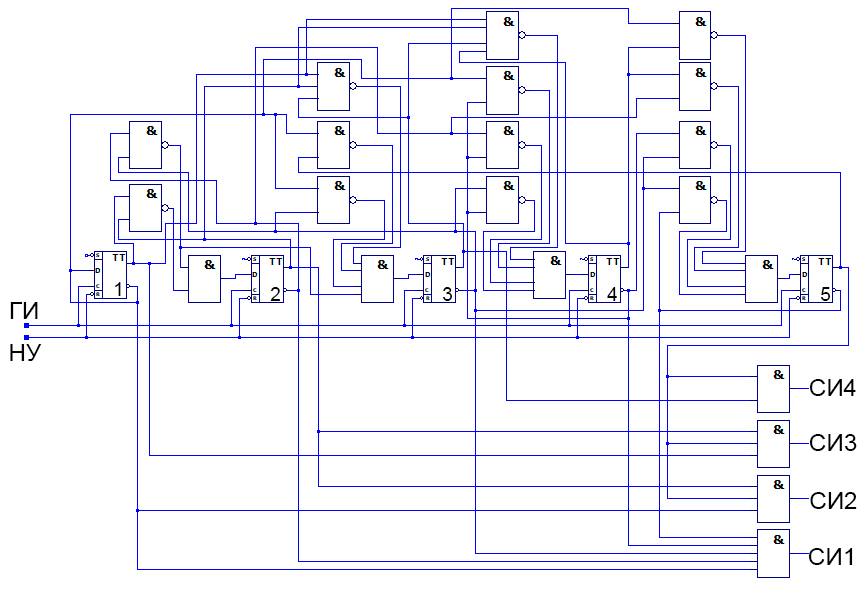
\includegraphics[width=0.8\linewidth]{images/gen_ch_sh}
	\caption{Логическая схема распредлителя сигналов}
	\label{fig:gen_ch_sh}
\end{figure}
\end{landscape}

\section{Общая структура схемы многоразрядного десятичного сумматора комбинационного типа с устройством управления}

\begin{figure}[H]
	\centering
	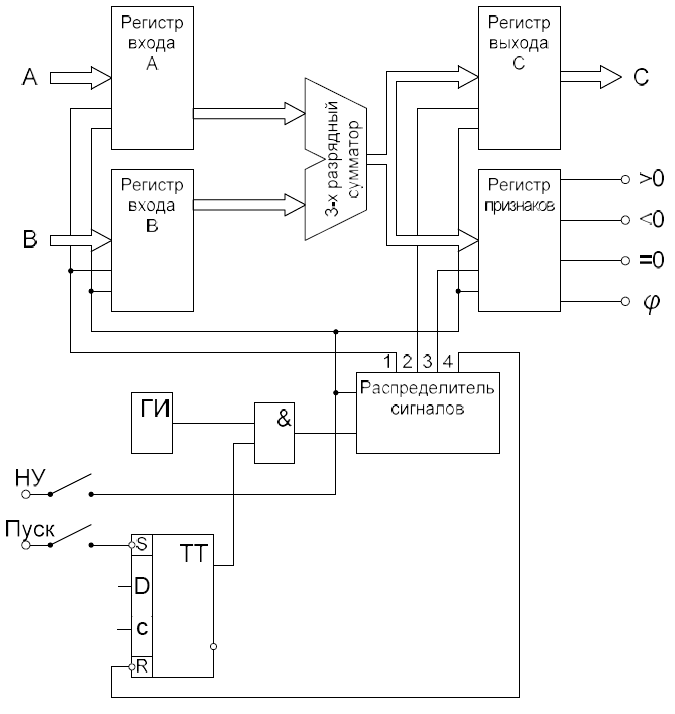
\includegraphics[width=1\linewidth]{images/itog_sh}
	\caption{Общая структура 3-х разрядного десятичного сумматора с устройством	управления}
	\label{fig:itog_sh}
\end{figure}

По сигналу НУ триггеры регистров и распределителя сигналов
устанавливаются в состояние "0". По сигналу «Пуск» триггер пуска
устанавливается в состояние "1" и импульсы с ГИ (генератор импульсов)
через схему "И" поступают на распределитель сигналов. Последний
вырабатывает управляющие сигналы СИ1, СИ2, СИ3 и СИ4. Сигнал СИ4
устанавливает триггер пуска в состояние "0" и отключает тем самым ГИ от
распределителя сигналов.


\section{Выводы по работе}

В ходе проделанной работы был спроектирован трехразрядный десятичный сумматор комбинационного типа в базисе И-НЕ, И на D-триггерах, двоично-десятичный код 2421. Были получены навыки работы с двоичной арифметикой, составления логических выражений и минимизация с помощью диаграмм Вейча и составление и минимизации функций переходов триггеров с помощью диаграмм Вейча.
\end{document}